\documentclass[11pt]{article}

%PRéAMBULE (packages)
\usepackage[T1]{fontenc}
\usepackage[utf8]{inputenc}
\usepackage[francais]{babel}
\usepackage[normalem]{ulem}
\usepackage{verbatim}
\usepackage[usenames,dvipsnames,table]{xcolor}
\usepackage{graphicx}
\usepackage{graphics}
\usepackage{fancyhdr}
\usepackage{amsfonts}
\usepackage{xcolor}
\usepackage{amsmath}
\usepackage{ulem}
\usepackage{adjustbox}
\usepackage{amssymb,amsmath,latexsym}
\usepackage{mathrsfs}
\usepackage[top=2cm, bottom=2cm, right=2cm, left=2cm, headheight=13.6pt]{geometry}
\usepackage{subfig}
\usepackage[bottom]{footmisc}
\usepackage{default}
\usepackage{hyperref}
\usepackage{lscape}
\usepackage[tikz]{bclogo}
\usepackage{verbatim}
\usepackage{listings}
\usepackage{tikz}
\usepackage[french]{minitoc}
\usepackage[numbered,framed]{mcode}
\usepackage{slashbox}
\usepackage{placeins}
\usepackage{lmodern}
%Pour lister le programme
%\lstset{
  %language=Pascal,
  %basicstyle=\small\sffamily,
  %breaklines=true,
  %columns=fullflexible
%}


%En-têtes et pieds de page
\fancypagestyle{mine}{ %
\fancyhf{}
\renewcommand\headrulewidth{0.2pt}
\fancyhead[R]{Pierre \textsc{Coieffey}~\\ Gautier \textsc{Darchen}}
\renewcommand\footrulewidth{0pt}
\fancyfoot[C]{\thepage}
\fancyfoot[L]{
\includegraphics[scale=0.2]{Insa.png}}
\fancyfoot[R]{\textsf{Projet de M8}}
}

\lstset{  breaklines=true,                % sets automatic line breaking
  breakatwhitespace=false,        % sets if automatic breaks should only happen}
}

\DeclareUnicodeCharacter{00A0}{ }

\pagestyle{fancy}
\renewcommand\headrulewidth{0.2pt}
\fancyhead[L]{\leftmark}
\fancyhead[R]{Pierre \textsc{Coieffey}~\\ Gautier \textsc{Darchen}}
\renewcommand\footrulewidth{0pt}
\fancyfoot[C]{\thepage}
\fancyfoot[L]{
\includegraphics[scale=0.2]{Insa.png}}
\fancyfoot[R]{\textsf{Projet de M8}}



\begin{document}

%Page de titre
\begin{titlepage}
\thispagestyle{empty}
\begin{figure}

\includegraphics[width=5cm]{Insa.png}\hfill
\end{figure}

\newcommand{\HRule}{\rule{\linewidth}{0.5mm}} 
\center 
\vspace*{\stretch{1}}\textsc{\huge Institut National des Sciences Appliqu\'{e}es de Rouen}\\[1.5cm] 
\textsc{\Large EC M8}\\[2cm] 

\HRule \\[0.4cm]
{ \huge \bfseries Rapport de projet de M8}\\[0.2cm] 
\HRule \\[2.5cm]
 
\LARGE \emph{\textbf{Titre du projet : }}\\
\LARGE{ \og Student performances \fg}\\
~\\

\Large{
Quels sont les principaux facteurs ayant une influence sur les résultats scolaires d'un élève ?\\ Quel est le degré d'influence de ces facteurs ?}\\[2cm] 


\large \emph{\textbf{Auteurs :}}\\
Pierre \textsc{Coieffey}\\
Gautier \textsc{Darchen}\\ 

~\\ ~\\[1cm]



\vfill{\today}\\[3cm]

\end{titlepage}

%Sommaire
\newpage

\tableofcontents

\newpage
\section*{Introduction}\addcontentsline{toc}{section}{Introduction}\thispagestyle{mine}
{\large ~\\

 Dans le cadre de notre projet de M8, il nous fallait trouver des données à traiter statistiquement afin d'appliquer dans un cadre pratique ce que nous avions de manière théorique. Nous souhaitions initialement traiter des données portant sur le sport. Cependant, les données que nous trouvions ne satisfaisaient pas toutes les conditions que nous nous étions fixés : grands échantillons, diversité des variables, plusieurs types d'études statistiques à réaliser... Après plusieurs semaines de recherches et l'accord de nos chargés de TD \--- Messieurs \textsc{Delporte}, \textsc{Canu} et \textsc{Rousselle} \--- nous nous sommes mis d'accord sur un sujet assez original : l'étude de notes d'élèves portugais\footnote{Ces données sont disponibles à l'adresse \url{https://archive.ics.uci.edu/ml/datasets/Student+Performance}.} dans différentes matières en fonction de multiples variables, liées à leur situation familiale, leurs habitudes de vie... ~\\\\

En premier lieu, nous nous sommes fixé comme objectif de cette étude statistique de répondre à notre problématique : Quels sont les principaux facteurs ayant une influence sur les résultats scolaires d’un élève ? Quel est le degré d’influence de ces facteurs ?~\\\\

Afin de répondre à cette problématique, nous allons tout d'abord présenter les données que nous avons étudiées, à savoir l'ensemble des variables, ainsi que les modalités que chacune d'entre elles représente. Ensuite, nous allons concrétiser le traitement statistique des données de sorte à en sortir dégager des conclusions, notamment sur le plan mathématique. Enfin, notre étude se complètera au travers de tests. Nous allons ainsi réaliser quelques tests de \textsc{Student} et tests du $\chi^2$. 
}





\newpage
\renewcommand*\lstlistingname{Code}
\renewcommand*{\lstlistlistingname}{Liste des codes}

\let\oldtabular=\tabular
\def\tabular{\scriptsize\oldtabular}

%%%%%%%%%%%%%%%%%%%%%%%%%%%%%%%%%%%%Partie 1
\section{Présentation et récupération des données}

Nous avons récupéré les données que nous avons choisi de traiter sur une librairie de données statistiques en ligne, à l'adresse \url{https://archive.ics.uci.edu/ml/datasets/Student+Performance}. Les données sont regroupées dans deux fichiers de type CSV (\emph{comma-separated values}).  Nous allons donc tout d'abord présenter les données, puis expliquer comment nous les avons récupérées afin de pouvoir les traiter de manière statistique.
~\\

\subsection{Présentation des données}
\subsubsection{Présentation globale}
Ces données décrivent les résultats d'étudiants de deux lycées au Portugal en fonction de certains critères. Les-dites données ont été rassemblées par le biais de questionnaires et de rapports réalisés par les écoles elles-mêmes. Parmi les critères, dont il nous faut déterminer les plus influents sur les résultats scolaires, figurent par exemple des caractéristiques démographiques, sociales  propres aux différents étudiants ou liées aux écoles. Deux bases de données sont fournies dans les fichiers CSV, permettant d'étudier les performances des élèves dans deux matières différentes : les mathématiques dans le fichier \texttt{student-mat.csv} et le portugais \--- qui est leur langue maternelle \--- dans le fichier \texttt{student-pro.csv}. Les deux lycées étudiés sont \textsc{Gabriel PEREIRA} et \textsc{Mousinho da SILVEIRA} et cette enquête date de fin 2014. Rassemblons dans un tableau les données concernant les 15 premiers élèves du fichier \texttt{student-mat.csv}, sachant que d'un fichier à l'autre, l'architecture des données est vraisemblablement la même si ce n'est que les résultats obtenus sont ceux d'une matière scolaire différente.
~\\\\\\\\\\

\begin{table}[h] \centering \caption{Première partie des données sur les 15 premiers individus du fichier \texttt{student-mat.csv}}
\begin{tabular}{|>{\columncolor{gray!40}\bfseries}r||c|c|c|c|c|c|c|c|c|c|c|}
  \hline
\rowcolor{gray!40}\bfseries Elève&\textbf{School}&\textbf{Sex}&\textbf{Age}&\textbf{Address}&\textbf{Famsize}&\textbf{Pstatus}&\textbf{Medu}&\textbf{Fedu}&\textbf{Mjob}&\textbf{Fjob}&\textbf{Reason}\\
  \hline
          
          1&GP&F&18&U&GT3&A&4&4&at\_home&teacher&course\\ \hline
          2&GP&F&17&U&GT3&T&1&1&at\_home&other&course\\ \hline
          3&GP&F&15&U&LE3&T&1&1&at\_home&other&other \\ \hline
          4&GP&F&15&U&GT3&T&4&2&health&services&home\\ \hline
          5&GP&F&16&U&GT3&T&3&3&other&other&home \\ \hline
          6&GP&M&16&U&LE3&T&4&3&services&other&reputation \\ \hline
          7&GP&M&16&U&LE3&T&2&2&other&other&home \\ \hline
          8&GP&F&17&U&GT3&A&4&4&other&teacher&home \\ \hline
          9&GP&M&15&U&LE3&A&3&2&services&other&home \\ \hline
          10&GP&M&15&U&GT3&T&3&4&other&other&home \\ \hline
          11&GP&F&15&U&GT3&T&4&4&teacher&health&reputation \\ \hline
          12&GP&F&15&U&GT3&T&2&1&services&other&reputation \\ \hline
          13&GP&M&15&U&LE3&T&4&4&health&services&course \\ \hline
          14&GP&M&15&U&GT3&T&4&3&teacher&other&course \\ \hline
          15&GP&M&15&U&GT3&A&2&2&other&other&home \\ \hline
\end{tabular}
\end{table}
~\\
%tab 2
\begin{table}[h] \centering \caption{Seconde partie des données sur les 15 premiers individus du fichier \texttt{student-mat.csv}}
\begin{tabular}{|>{\columncolor{gray!40}\bfseries}r||c|c|c|c|c|c|c|c|c|}
  \hline
\rowcolor{gray!40}\bfseries Elève&\textbf{Guardian}&\textbf{Traveltime}&\textbf{Studytime}&\textbf{Failures}&\textbf{Schoolsup}&\textbf{Famsup}&\textbf{Paid}&\textbf{Activities}&\textbf{Nursery}\\
  \hline
          1&mother&2&2&0&yes&no&no&no&yes \\ \hline
          2&father&1&2&0&no&yes&no&no&no\\ \hline
          3&mother&1&2&3&yes&no&yes&no&yes \\ \hline
          4&mother&1&3&0&no&yes&yes&yes&yes\\ \hline
          5&father&1&2&0&no&yes&yes&no&yes \\ \hline
          6&mother&1&2&0&no&yes&yes&yes&yes \\ \hline
          7&mother&1&2&0&no&no&no&no&yes \\ \hline
          8&mother&2&2&0&yes&yes&no&no&yes \\ \hline
          9&mother&1&2&0&no&yes&yes&no&yes \\ \hline
          10&mother&1&2&0&no&yes&yes&yes&yes \\ \hline
          11&mother&1&2&0&no&yes&yes&no&yes \\ \hline
          12&father&3&3&0&no&yes&no&yes&yes \\ \hline
          13&father&1&1&0&no&yes&yes&yes&yes \\ \hline
          14&mother&2&2&0&no&yes&yes&no&yes \\ \hline
          15&other&1&3&0&no&yes&no&no&yes \\ \hline
\end{tabular}
\end{table}
~\\

\begin{table}[h] \centering \caption{Troisième partie des données sur les 15 premiers individus du fichier \texttt{student-mat.csv}}
\begin{tabular}{|>{\columncolor{gray!40}\bfseries}r||c|c|c|c|c|c|c|c|c|c|c|}
  \hline
\rowcolor{gray!40}\bfseries Elève&\textbf{Higher}&\textbf{Internet}&\textbf{Romantic}&\textbf{Famrel}&\textbf{Freetime}&\textbf{Goout}&\textbf{Dalc}&\textbf{Walc}&\textbf{Health}&\textbf{Absences}\\
  \hline
          1&yes&no&no&4&3&4&1&1&3&6\\ \hline
          2&yes&yes&no&5&3&3&1&1&3&4\\ \hline
          3&yes&yes&no&4&3&2&2&3&3&10\\ \hline
          4&yes&yes&yes&3&2&2&1&1&5&2\\ \hline
          5&yes&no&no&4&3&2&1&2&5&4 \\ \hline
          6&yes&yes&no&5&4&2&1&2&5&10 \\ \hline
          7&yes&yes&no&4&4&4&1&1&3&0\\ \hline
          8&yes&no&no&4&1&4&1&1&1&6 \\ \hline
          9&yes&yes&no&4&2&2&1&1&1&0 \\ \hline
          10&yes&yes&no&5&5&1&1&1&5&0 \\ \hline
          11&yes&yes&no&3&3&3&1&2&2&0 \\ \hline
          12&yes&yes&no&5&2&2&1&1&4&4 \\ \hline
          13&yes&yes&no&4&3&3&1&3&5&2 \\ \hline
          14&yes&yes&no&5&4&3&1&2&3&2 \\ \hline
          15&yes&yes&yes&4&5&2&1&1&3&0 \\ \hline
\end{tabular}
\end{table}

\begin{table}[h!] \centering \caption{Quatrième partie des données sur les 15 premiers individus du fichier \texttt{student-mat.csv}}
\begin{tabular}{|>{\columncolor{gray!40}\bfseries}r||c|c|c|}
  \hline
\rowcolor{gray!40}\bfseries Elève&\textbf{G1}&\textbf{G2}&\textbf{G3}\\
  \hline
          1&5&6&6\\ \hline
          2&5&5&6\\ \hline
          3&7&8&10\\ \hline
          4&15&14&15\\ \hline
          5&6&10&10 \\ \hline
          6&15&15&15 \\ \hline
          7&12&12&11\\ \hline
          8&6&5&6 \\ \hline
          9&16&18&19\\ \hline
          10&14&15&15 \\ \hline
          11&10&8&9\\ \hline
          12&10&12&12 \\ \hline
          13&14&14&14\\ \hline
          14&10&10&11 \\ \hline
          15&14&16&16\\ \hline
\end{tabular}
\end{table}





\subsubsection{Description des variables}
Les deux fichiers CSV contiennent les données de 33 variables : 32 sont explicatives et la 33$^{\text{ème}}$ variable représente les notes que pourraient obtenir les élèves au troisième trimestre et est donc la variable à expliquer. Décrivons chacune d'entre elles en détail. 


\renewcommand{\labelenumi}{\textbf{\theenumi.}}
\renewcommand{\labelenumii}{\textbf{\theenumii.}}
\renewcommand{\theenumi}{\arabic{enumi}}
\renewcommand{\theenumii}{\alph{enumii}}
\begin{enumerate}
\item \textbf{\emph{School}} \--- L'école de l'individu concerné.
	\\\textsf{Valeurs binaires : }\begin{itemize}
	\item[\textbullet] \og GP \fg~ pour \textsc{Gabriel PEREIRA};
	\item[\textbullet] \og MS \fg~ pour \textsc{Mousinho da SILVEIRA}.
	\end{itemize}

\item \textbf{\emph{Sex}} \--- Le sexe de l'individu concerné.
	\\\textsf{Valeurs binaires : }\begin{itemize}
	\item[\textbullet] \og F \fg~pour féminin ;
	\item[\textbullet] \og M \fg~pour masculin.
	\end{itemize}

\item \textbf{\emph{Age}} \--- L'âge de l'étudiant concerné.
	\\\textsf{Valeurs numériques allant de 15 à 22 ans}.

\item \textbf{\emph{Address}} \--- Le lieu de vie de l'individu concerné.
	\\\textsf{Valeurs binaires : }\begin{itemize}
	\item[\textbullet] \og U \fg~ pour un mode de vie urbain;
	\item[\textbullet] \og R >> pour un mode de vie rural.
	\end{itemize}

\item  \textbf{\emph{Famsize}} \--- La taille de la famille de l'individu concerné.
	\\\textsf{Valeurs binaires : }\begin{itemize}
	\item[\textbullet] << LE3 >>  pour \emph{less or equal to 3};
	\item[\textbullet] << GT3 >> pour \emph{greater than 3}.
	\end{itemize}


\item \textbf{\emph{Pstatus}} \--- Le statut de cohabitation des parents de l'individu concerné.
	\\\textsf{Valeurs binaires : }\begin{itemize}
	\item[\textbullet] << T >> pour \emph{living together} ;
	\item[\textbullet] << A >> pour \emph{apart}).
	\end{itemize}

\item \textbf{\emph{Medu}} \--- \label{rap1}Le niveau d'éducation de la mère de l'individu concerné. 
	\\\textsf{Valeurs numériques : }\begin{itemize}
	\item[\textbullet] 0 si la mère n'est pas allée à l'école ;
	\item[\textbullet] 1 si elle a passé moins de 4 ans à l'école (primaire) ;
	\item[\textbullet] 2 si elle a passé entre 5 et 9 ans à l'école (fin primaire et collège) ;
	\item[\textbullet] 3 si la mère a eu une éducation secondaire\footnote{Dans le système scolaire portugais, il s'agit de l'équivalent du Lycée en France.} (lycée) ;
	\item[\textbullet] 4 si elle est allée dans des écoles d'enseignement supérieur.
	\end{itemize}

\item \textbf{\emph{Fedu}} \--- Le niveau d'éducation du père de l'individu concerné.
	\\\textsf{Valeurs numériques : }\begin{itemize}
	\item[\textbullet] 0 si le père n'est pas allé à l'école ;
	\item[\textbullet] 1 si le père a passé moins de 4 ans à l'école (primaire) ;
	\item[\textbullet] 2 si le père a passé entre 5 et 9 ans à l'école (fin primaire et collège) ;
	\item[\textbullet] 3 si le père a eu une éducation secondaire (lycée) ;
	\item[\textbullet] 4 si il est allé dans des écoles d'enseignement supérieur.
	\end{itemize}

\item \textbf{\emph{Mjob}} \--- \label{rap2} Le métier de la mère de l'individu concerné.
	\\\textsf{Valeurs nominales : }\begin{itemize}
	\item[\textbullet] << \emph{teacher} >> si elle travaille dans l'enseignement ;
	\item[\textbullet] << \emph{health} >> si elle travaille dans le domaine de la santé ;
	\item[\textbullet] << \emph{services} >> si elle travaille dans les services publics (par exemple dans  l'administratif ou la police) ;
	\item[\textbullet] << \emph{at\_home} >> si elle est femme au foyer ;
	\item[\textbullet] << \emph{other} >> si son métier ne rentre dans aucune de ces catégories.
	\end{itemize}

\item \textbf{\emph{Fjob}} \--- Le métier du père de l'individu concerné.
	\\\textsf{Valeurs nominales : }\begin{itemize}
	\item[\textbullet] << \emph{teacher} >> si il travaille dans l'enseignement ;
	\item[\textbullet] << \emph{health} >> si il travaille dans le domaine de la santé ;
	\item[\textbullet] << \emph{services} >> si il travaille dans les services publics (par exemple dans  l'administratif ou la police) ;
	\item[\textbullet] << \emph{at\_home} >> si il est homme au foyer ;
	\item[\textbullet] << \emph{other} >> si son métier ne rentre dans aucune de ces catégories.
	\end{itemize}

\item \textbf{\emph{Reason}} \--- La raison pour laquelle l'individu concerné a choisi l'école dans laquelle il étudie. 
	\\\textsf{Valeurs nominales : }\begin{itemize}
	\item[\textbullet] << \emph{home} >> si ce choix est dû à la proximité de l'école avec la maison ;
	\item[\textbullet] << \emph{reputation} >> si c'est grâce à la réputation de l'école ;
	\item[\textbullet] << \emph{course} >> si ce choix est dû à l'intérêt pour les matières enseignées par l'école ;
	\item[\textbullet] << \emph{other} >> si le choix est dû à un autre critère.
	\end{itemize}

\item \textbf{\emph{Guardian}} \--- Le responsable légal ou personne qui s'occupe de l'individu concerné. 
	\\\textsf{Valeurs nominales : }\begin{itemize}
	\item[\textbullet] << \emph{mother} >> si le tutrice est la mère ;
	\item[\textbullet] << \emph{father} >> si le tuteur est le père ;
	\item[\textbullet] << \emph{other} >> s'il s'agit d'une autre personne.
	\end{itemize}

 \item \textbf{\emph{Traveltime}} \--- Le temps de trajet moyen entre l'école et le domicile de l'étudiant concerné. 
	\\\textsf{Valeurs numériques : }\begin{itemize}
	\item[\textbullet] 1 si le trajet dure en moyenne moins de 15 minutes ;
	\item[\textbullet] 2 si le trajet dure en moyenne entre 15 et 30 minutes ;
	\item[\textbullet] 3 si le trajet dure en moyenne entre 30 minutes et une heure;
	\item[\textbullet] 4 si le trajet dure en moyenne plus d'une heure.
	\end{itemize}

\item \textbf{\emph{Studytime}} \--- Le temps que passe l'élève concerné chaque semaine sur son travail personnel (révisions). 
	\\\textsf{Valeurs numériques : }\begin{itemize}
	\item[\textbullet] 1 s'il étudie en moyenne moins de 2 heures par semaine ;
	\item[\textbullet] 2 s'il étudie en moyenne entre 2 et 5 heures par semaine ;
	\item[\textbullet] 3 s'il étudie en moyenne entre 5 et 10 heures par semaine ;
	\item[\textbullet] 4 s'il étudie en moyenne plus de 10 heures par semaine.
	\end{itemize}
	
\item \textbf{\emph{Failures}} \--- Le nombre de classes que l'individu a redoublé par le passé. 
	\\\textsf{Valeurs numériques : }\begin{itemize}
	\item[\textbullet] $n$, avec $1\leq n <3$ si l'élève a redoublé $n$ classe(s) ;
	\item[\textbullet] 4 si l'élève a redoublé plus de 3 fois.
	\end{itemize}

\item \textbf{\emph{Schoolsup}} \--- Un booléen décrivant si l'individu dispose d'un soutien éducatif supplémentaire (dans l'école). 
	\\\textsf{Valeurs binaires (booléen) : }\begin{itemize}
	\item[\textbullet] \emph{yes} si l'individu dispose d'un soutien au sein de l'école ;
	\item[\textbullet] \emph{no} sinon.
	\end{itemize}

\item \textbf{\emph{Famsup}} \--- Un booléen décrivant si l'individu dispose d'un soutien pédagogique familial. 
	\\\textsf{Valeurs binaires (booléen) : }\begin{itemize}
	\item[\textbullet] \emph{yes} si l'individu dispose d'un soutien pédagogique familial ;
	\item[\textbullet] \emph{no} sinon.
	\end{itemize}
	
\item \textbf{\emph{Paid}} \--- Un booléen décrivant si l'individu prend des cours particuliers (payants) dans l'une des deux matières étudiées (mathématiques ou portugais). 
	\\\textsf{Valeurs binaires (booléen) : }\begin{itemize}
	\item[\textbullet] \emph{yes} si l'individu prend des cours particuliers payants;
	\item[\textbullet] \emph{no} sinon.
	\end{itemize}

\item \textbf{\emph{Activities}} \--- Un booléen décrivant si l'individu pratique des activités extra-scolaires. 
	\\\textsf{Valeurs binaires (booléen) : }\begin{itemize}
	\item[\textbullet] \emph{yes} si l'individu pratique au moins une activité extra-scolaire;
	\item[\textbullet] \emph{no} sinon.
	\end{itemize}
	
\item \textbf{\emph{Nursery}} \--- Un booléen décrivant si l'individu est allé à l'école maternelle. 
	\\\textsf{Valeurs binaires (booléen) : }\begin{itemize}
	\item[\textbullet] \emph{yes} si l'individu est allé à la maternelle;
	\item[\textbullet] \emph{no} sinon.
	\end{itemize}
	
\item \textbf{\emph{Higher}} \--- Un booléen décrivant si l'individu a pour intention, au moment de l'enquête, de faire des études supérieures. 
	\\\textsf{Valeurs binaires (booléen) : }\begin{itemize}
	\item[\textbullet] \emph{yes} si l'individu a pour intention de faire des études supérieures;
	\item[\textbullet] \emph{no} sinon.
	\end{itemize}
	
\item \textbf{\emph{Internet}} \--- Un booléen décrivant si l'individu a un accès à Internet à son domicile. 
	\\\textsf{Valeurs binaires (booléen) : }\begin{itemize}
	\item[\textbullet] \emph{yes} si possède un accès à Internet chez lui;
	\item[\textbullet] \emph{no} sinon.
	\end{itemize}
	
\item \textbf{\emph{Romantic}} \--- Un booléen décrivant si l'individu est en couple ou non. 
	\\\textsf{Valeurs binaires (booléen) : }\begin{itemize}
	\item[\textbullet] \emph{yes} si l'individu est en couple au moment de l'enquête;
	\item[\textbullet] \emph{no} sinon.
	\end{itemize}
	
\item \textbf{\emph{Famrel}} \--- Une valeur décrivant la qualité de la relation entre l'individu et les membres de sa famille. 
	\\\textsf{Valeurs numériques (de 1 à 5) : }\begin{itemize}
	\item[\textbullet] 1 si les relations sont très mauvaises ;
	\item[$\vdots$] 
	\item[\textbullet] 5 si ces relations sont excellentes.
	\end{itemize}
	
\item \textbf{\emph{Freetime}} \--- Une valeur décrivant le temps libre dont dispose l'étudiant après les cours. 
	\\\textsf{Valeurs numériques (de 1 à 5) : }\begin{itemize}
	\item[\textbullet] 1 si l'étudiant a très peu de temps libre après les cours ;
	\item[$\vdots$] 
	\item[\textbullet] 5 si l'étudiant a beaucoup de temps libre après les cours.
	\end{itemize}
	
\item \textbf{\emph{Goout}} \--- Une valeur numérique décrivant le temps que l'élève passe avec ses amis hors de chez lui. 
	\\\textsf{Valeurs numériques (de 1 à 5) : }\begin{itemize}
	\item[\textbullet] 1 si l'élève sort très peu avec ses amis ;
	\item[$\vdots$] 
	\item[\textbullet] 5 si l'élève sort beaucoup avec ses amis.
	\end{itemize}
	
\item \textbf{\emph{Dalc}} \--- \label{rap3} Une valeur numérique représentant la quantité d'alcool que consomme l'étudiant quotidiennement. 
	\\\textsf{Valeurs numériques (de 1 à 5) : }\begin{itemize}
	\item[\textbullet] 1 si l'étudiant consomme très peu d'alcool au quotidien ;
	\item[$\vdots$] 
	\item[\textbullet] 5 si l'étudiant consomme beaucoup d'alcool au quotidien.
	\end{itemize}
	
\item \textbf{\emph{Walc}} \--- Une valeur numérique représentant la quantité d'alcool que consomme l'étudiant chaque semaine. 
	\\\textsf{Valeurs numériques (de 1 à 5) : }\begin{itemize}
	\item[\textbullet] 1 si l'étudiant consomme très peu d'alcool par semaine ;
	\item[$\vdots$] 
	\item[\textbullet] 5 si l'étudiant consomme beaucoup d'alcool par semaine.
	\end{itemize}

\item \textbf{\emph{Health}} \--- Une valeur numérique représentant l'état de santé de l'étudiant au moment de l'enquête (santé physique et/ou psychologique). 
	\\\textsf{Valeurs numériques (de 1 à 5) : }\begin{itemize}
	\item[\textbullet] 1 si l'étudiant était en très mauvaise santé au moment de l'enquête;
	\item[$\vdots$] 
	\item[\textbullet] 5 si l'étudiant était en excellente santé au moment de l'enquête.
	\end{itemize}
	
\item \textbf{\emph{Absences}} \--- Le nombre de jours durant lesquels l'élève a été absent. 
	\\\textsf{Valeurs numériques (de 0 à 93) : }\begin{itemize}
	\item[\textbullet] 0 si l'élève n'a jamais été absent durant l'année de l'enquête;
	\item[$\vdots$] 
	\item[\textbullet] 93 si l'élève a été absent 93 fois pendant l'année (il s'agit de la valeur maximale d'absentéisme dans cette enquête).
	\end{itemize}
	
\item \textbf{\emph{G1}} \--- La note finale de l'étudiant à la fin du premier trimestre dans la matière en question (mathématiques ou portugais). 
	\\\textsf{Valeurs numériques (de 0 à 20) : }\begin{itemize}
	\item[\textbullet] 0 : note minimale;
	\item[$\vdots$] 
	\item[\textbullet] 20 : note maximale.
	\end{itemize}
	
\item \textbf{\emph{G2}} \--- La note finale de l'étudiant à la fin du second trimestre dans la matière en question (mathématiques ou portugais). 
	\\\textsf{Valeurs numériques (de 0 à 20) : }\begin{itemize}
	\item[\textbullet] 0 : note minimale;
	\item[$\vdots$] 
	\item[\textbullet] 20 : note maximale.
	\end{itemize}


\item \textbf{\emph{G3}} \--- La note finale de l'étudiant à la fin du troisième trimestre dans la matière en question (mathématiques ou portugais). Il s'agit de l' << \emph{output target} >>, autrement dit, la variable à expliquer.
	\\\textsf{Valeurs numériques (de 0 à 20) : }\begin{itemize}
	\item[\textbullet] 0 : note minimale;
	\item[$\vdots$] 
	\item[\textbullet] 20 : note maximale.
	\end{itemize}
	
\end{enumerate}
\renewcommand{\labelenumi}{\theenumi.}
\renewcommand{\labelenumii}{\theenumii.}
\renewcommand{\theenumi}{\arabic{enumi}}
\renewcommand{\theenumii}{\alph{enumii}}

\subsection{Récupération des données}

Les données sont stockées dans des fichiers CSV. Nous décrirons ici la manière dont nous avons extrait les données du fichier \texttt{student-mat.csv}, sachant que nous avons procédé exactement de la même façon pour le fichier \texttt{student-por.csv}. Le code de cette extraction est réalisé dans le fichier \texttt{DonneesProjetM8.m}.
~\\

La première étape consiste à charger une matrice contenant les données. Pour les importer et pouvoir les exploiter avec le logiciel \emph{Matlab}, nous avons donc tout d'abord dû utiliser la fonction \texttt{csvimport}. Ainsi, la première ligne de code de cette extraction est :

\begin{lstlisting}[firstnumber=2,caption={Extraction des données du fichier CSV dans une matrice de \texttt{cell}}]
dataMat=csvimport('student-mat.csv');
\end{lstlisting}
~\\

Nous avons alors la matrice \texttt{dataMat} qui est de type \texttt{cell}. Il faut donc convertir ces valeurs afin de pouvoir les exploiter. Cependant, il ne faut pas oublier que les variables ont des types différents. En effet, comme nous l'avons vu précédemment, certaines variables admettent des modalités nominales, d'autres des modalités numériques... 

Ainsi, nous convertissons les données de type \texttt{cell} dont nous voulons obtenir des valeurs numériques. Toutes les variables obtenues par le code suivant seront alors de type \texttt{double} et nous pourrons les exploiter.

\begin{lstlisting}[firstnumber=4,caption={Transformation de \texttt{cell} en \texttt{double}}]
% Donnees numeriques
Mat_Age=cell2mat(dataMat(2:end,3));
Mat_Medu=cell2mat(dataMat(2:end,7));
Mat_Fedu=cell2mat(dataMat(2:end,8));
Mat_Traveltime=cell2mat(dataMat(2:end,13));
Mat_Studytime=cell2mat(dataMat(2:end,14));
Mat_Failures=cell2mat(dataMat(2:end,15));
Mat_Famrel=cell2mat(dataMat(2:end,24));
Mat_Freetime=cell2mat(dataMat(2:end,25));
Mat_Goout=cell2mat(dataMat(2:end,26));
Mat_Dalc=cell2mat(dataMat(2:end,27));
Mat_Walc=cell2mat(dataMat(2:end,28));
Mat_Health=cell2mat(dataMat(2:end,29));
Mat_Absences=cell2mat(dataMat(2:end,30));
Mat_G1=cell2mat(dataMat(2:end,31));
Mat_G2=cell2mat(dataMat(2:end,32));
Mat_G3=cell2mat(dataMat(2:end,33));
\end{lstlisting}

Par ailleurs, nous voulons que certaines variables, comme celle indiquant le métier de la mère d'un élève par exemple, soient de type \text{char} puisqu'elles représentent des chaînes de caractères. C'est alors tout l'intérêt du code qui suit.

\begin{lstlisting}[firstnumber=22,caption={Transformation de \texttt{cell} en \texttt{char}}]
% Donnees en chaines de caracteres
Mat_School=char(dataMat(2:end,1));
Mat_Sex=char(dataMat(2:end,2));
Mat_Address=char(dataMat(2:end,4));
Mat_Famsize=char(dataMat(2:end,5));
Mat_Pstatus=char(dataMat(2:end,6));
Mat_Mjob=char(dataMat(2:end,9));
Mat_Fjob=char(dataMat(2:end,10));
Mat_Reason=char(dataMat(2:end,11));
Mat_Guardian=char(dataMat(2:end,12));
Mat_Schoolsup=char(dataMat(2:end,16));
Mat_Famsup=char(dataMat(2:end,17));
Mat_Paid=char(dataMat(2:end,18));
Mat_Activities=char(dataMat(2:end,19));
Mat_Nursery=char(dataMat(2:end,20));
Mat_Higher=char(dataMat(2:end,21));
Mat_Internet=char(dataMat(2:end,22));
Mat_Romantic=char(dataMat(2:end,23));
\end{lstlisting}

A ce stade, nous réalisons exactement les mêmes transformations pour les données contenues dans le fichier \texttt{student-por.csv}.

Ensuite, il faut ranger les données de type \texttt{char} en valeurs numériques. On associe alors une valeur numérique à une modalité en chaîne de caractères. Les différentes valeurs numériques associées aux modalités d'une variable sont indiquées dans le code qui suit.

\begin{lstlisting}[firstnumber=87, caption={Extrait du rangement des modalités de type \texttt{char} avec des valeurs numériques de type \texttt{double}}]
%% Rangement modalites (chaines) fichier 'student_mat.csv'

%Rangement modalites Mat_School (0=MS / 1=GP)
TabModMat_School=ones(length(Mat_School),1);
for i=1:length(Mat_School)
    ind=[];
    if (Mat_School(i,:)=='MS')
       ind=[ind ;i];
       TabModMat_School(ind,1)=0;
    end
end

%Rangement modalites Mat_Sex (0=F / 1=M)
TabModMat_Sex=ones(length(Mat_Sex),1);
for i=1:length(Mat_Sex)
    ind=[];
    if (Mat_Sex(i,:)=='F')
       ind=[ind ;i];
       TabModMat_Sex(ind,1)=0;
    end
end

%Rangement modalites Mat_Address (0=U / 1=R)
TabModMat_Address=ones(length(Mat_Address),1);
for i=1:length(Mat_Address)
    ind=[];
    if (Mat_Address(i,:)=='U')
       ind=[ind ;i];
       TabModMat_Address(ind,1)=0;
    end
end

%Rangement modalites Mat_Famsize (0=LE3 / 1=GT3)
TabModMat_Famsize=ones(length(Mat_Famsize),1);
for i=1:length(Mat_Famsize)
    ind=[];
    if (Mat_Famsize(i,:)=='LE3')
       ind=[ind ;i];
       TabModMat_Famsize(ind,1)=0;
    end
end

%Rangement modalites Mat_Pstatus (0=A / 1=T)
TabModMat_Pstatus=ones(length(Mat_Pstatus),1);
for i=1:length(Mat_Pstatus)
    ind=[];
    if (Mat_Pstatus(i,:)=='A')
       ind=[ind ;i];
       TabModMat_Pstatus(ind,1)=0;
    end
end

%Rangement modalites Mat_Mjob (0=at_home / 1=health / 2=other / 3=services / 4=teacher)
TabModMat_Mjob=ones(length(Mat_Mjob),1);
for i=1:length(Mat_Mjob)
    ind=[];
    if (Mat_Mjob(i,:)=='at_home ')
       ind=[ind ;i];
       TabModMat_Mjob(ind,1)=0;
    end
    if (Mat_Mjob(i,:)=='other   ')
       ind=[ind ;i];
       TabModMat_Mjob(ind,1)=2;
    end
    if (Mat_Mjob(i,:)=='services')
       ind=[ind ;i];
       TabModMat_Mjob(ind,1)=3;
    end
    if (Mat_Mjob(i,:)=='teacher ')
       ind=[ind ;i];
       TabModMat_Mjob(ind,1)=4;
    end
end

%Et ainsi de suite pour toutes les autres variables et l'autre fichier
\end{lstlisting}

A ce stade, les données sont rangées et il nous reste à les traiter statistiquement. Ce traitement se fera dans un autre fichier \texttt{Traitement.m} qui fera appel au fichier \texttt{DonneesProjetM8.m} que nous venons d'analyser. 


\newpage
\section{Traitement des données}
\subsection{Etude des notes finales des élèves}

Dans un premier temps, nous avons décidé de traiter la variable des notes finales des élèves toute seule pour nous familiariser un peu plus avec le sujet.

\begin{figure}[h]
\centering
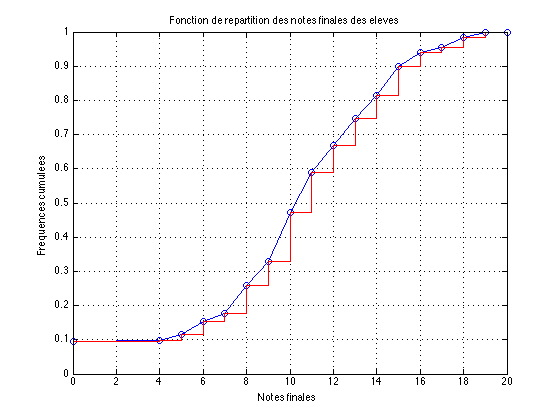
\includegraphics[scale=0.5]{Images/fig1.png}
\caption{Fonction de répartition des notes finales des élèves}

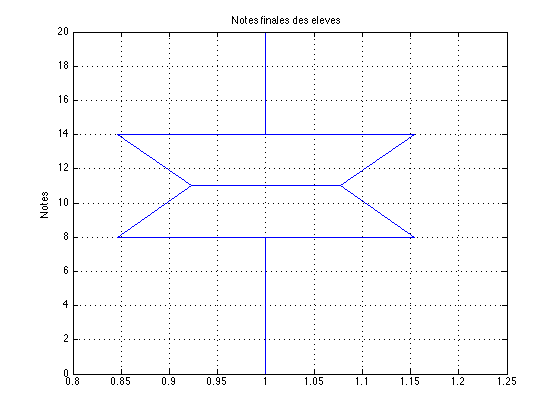
\includegraphics[scale=0.5]{Images/fig2.png}
\caption{Boîte à moustache des notes finales des élèves}
\end{figure}

\begin{figure}[h]
\centering
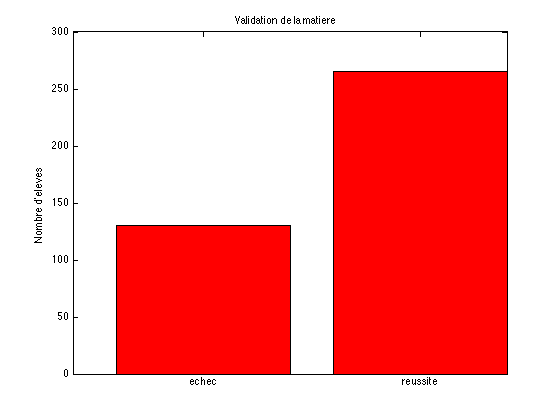
\includegraphics[scale=0.5]{Images/fig3.png}
\caption{Histogramme des élèves validant la matière Mathématiques}

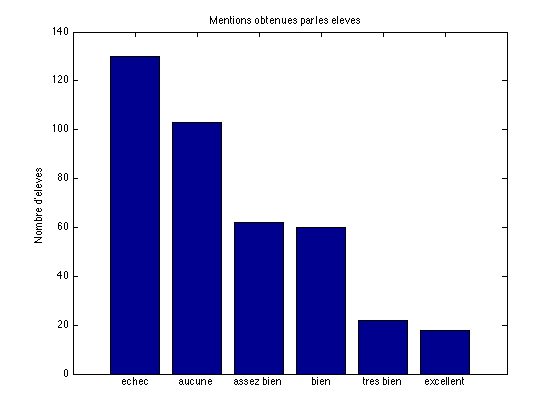
\includegraphics[scale=0.5]{Images/fig4.png}
\caption{Histogramme des mentions obtenues par les élèves}
\end{figure}

\FloatBarrier
On remarque donc grâce à ces quelques graphiques que le taux d'échec des élèves dans cette matière paraît plutôt élevé avec 32,91\% d'élèves ne validant pas leur année. Cependant ce chiffre doit être relativisé étant donné qu'il ne concerne qu'une seule matière. Les principaux indicateurs de cet échantillon de notes sont quant à eux plutôt \og normaux \fg{} avec une moyenne de 10.42, une médiane de 11, un premier quartile égal à 8 et un troisième égal à 14, pour une distance inter-quartiles de 6, et avec des notes occupant toute l'échelle de notation. En effet, la notation adoptée tend à suivre une courbe de \textsc{Gauss} c'est-à-dire qu'il y a beaucoup de notes moyennes pour très peu de notes extrêmes comme le montrent les mentions obtenues par les élèves.

Après avoir étudié ces notes finales, il est à présent temps de revenir à la problématique de notre sujet et de nous intéresser aux variables influençant cette fameuse note finale. Et pour ce faire, nous allons réaliser une Analyse en Composantes Principales (ACP) qui nous permettra d'avoir une vue d'ensemble sur toutes les variables pouvant influencer positivement ou négativement les notes finales des élèves.

\subsection{Analyse en Composantes Principales}
La première chose à faire dans une ACP est de centrer et réduire les données pour éviter que des variables possédant des modalités très élevées prennent le pas sur d'autres ayant des modalités très faibles. 
\begin{lstlisting}[firstnumber=62]
Xc_Mat=(X_Mat-moyenne);% matrice centree
Xn_Mat=Xc_Mat./ecart_type;% matrice centree et reduite
\end{lstlisting}

La deuxième étape, quant à elle, consiste à calculer les vecteurs et valeurs propres de cette matrice.
\begin{lstlisting}[firstnumber=65]
[V D]=eig(Xn_Mat'*Xn_Mat);% calcul des vecteurs et valeurs propres
lambda=diag(D);% valeurs propres
\end{lstlisting}

Une fois cette étape réalisée, il faut calculer le pourcentage d'information porté par chacune de nos valeurs propres. Malheureusement, comme nous avons de très nombreuses variables, les pourcentages portés par chacune de nos valeurs propres vont être assez faibles et par conséquent notre ACP ne va pas pas être en mesure de représenter plus d'un quart des informations. Cependant, cette analyse va quand même nous permettre d'avoir une vue d'ensemble des corrélations entre variables et va nous permettre d'orienter la suite de notre traitement de données.


\begin{table}[h] \centering \caption{Valeurs propres et pourcentages d'information}
\begin{tabular}{|c|c|}
  \hline
\rowcolor{gray!40}\bfseries $\lambda$ &\textbf{Pourcentage d'information}\\
  \hline
          30.572  &    0.23514\\\hline
       64.432     & 0.49555\\\hline
       109.57     & 0.84272\\\hline
       118.98      &0.91509\\\hline
       156.61       &1.2045\\\hline
       180.52       &1.3884\\\hline
       194.99       &1.4997\\\hline
       210.82       &1.6214\\\hline
       220.43       &1.6954\\\hline
       234.49       &1.8035\\\hline
        247.9       &1.9067\\\hline
       252.05      & 1.9386\\\hline
       277.56       &2.1348\\\hline
       282.37      & 2.1717\\\hline
       300.06     &  2.3078\\\hline
       314.17      & 2.4163\\\hline
       315.76       &2.4286\\\hline
       331.84       &2.5522\\\hline
        358.1     &  2.7542\\\hline
       376.58     &  2.8963\\\hline
       381.59      & 2.9349\\\hline
       401.41       &3.0873\\\hline
       422.88       &3.2525\\\hline
       436.22        &3.355\\\hline
       471.01      & 3.6226\\\hline
       489.44       &3.7643\\\hline
       550.89      & 4.2369\\\hline
       564.17       &4.3391\\\hline
       600.73       &4.6203\\\hline
        701.2        &5.393\\\hline
       878.27       &6.7548\\\hline
       1000.4       &7.6945\\\hline
         1526       &11.736\\\hline
\end{tabular}
\end{table}

Enfin, la dernière étape est de visualiser les variables en les projetant sur les vecteurs propres associés aux plus grandes valeurs propres. Ici nous avons choisi les 2 plus grandes après avoir conclu que l'ajout de la troisième n'apportait rien de plus si ce n'est une visualisation plus complexe.
De même, nous avons remarqué que la visualisation des individus n'apportait rien à l'analyse. En effet, le fait d'avoir un nombre très important d'individus dans notre base de données rendait la visualisation brouillonne et ne permettait pas de tirer un quelconque enseignement de cette analyse.

\begin{figure}[h]
\centering
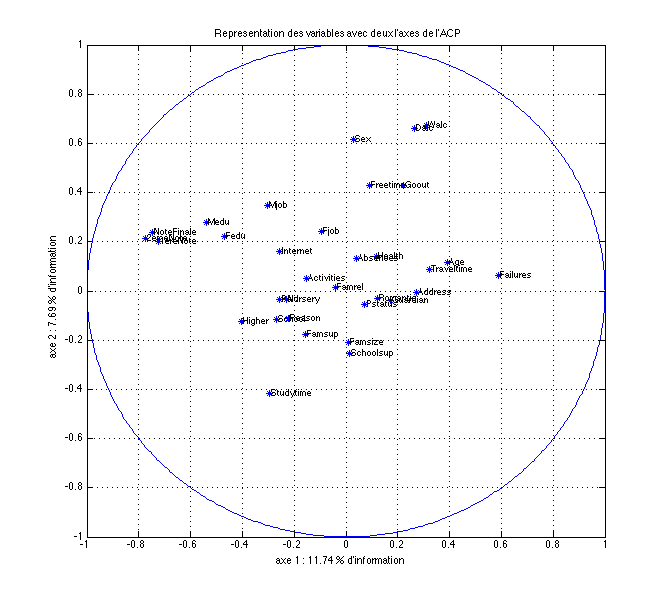
\includegraphics[scale=0.7]{Images/fig5.png}
\caption{Résultat de l'ACP après projection sur les composantes principales}
\end{figure}

On peut voir sur ce graphique que les première et deuxième notes sont très fortement corrélées positivement avec la note finale. Ceci est logique étant donné que ces trois variables sont du même type et cela signifie que si les premières et deuxième notes sont élevées, la note finale le sera également (et inversement). Nous essayerons donc, sachant cela, de prédire la note finale à l'aide des deux premières. Concernant les autres variables pouvant avoir une influence sur la note finale, nous retrouvons \texttt{Medu} et \texttt{Fedu} corrélées positivement avec la note finale mais également \texttt{Failures} et \texttt{Age} corrélées négativement. Tout cela signifie que plus l'éducation des parents est forte et plus la note finale sera élevée (et inversement) contrairement aux deux autres variables qui indiquent que plus les absences et les âges sont élevés et plus la note finale sera faible (et inversement). Bien-entendu, ces conclusions ne sont qu'intermédiaires et elles demanderont à être vérifiées par la suite pour voir si oui ou non ces variables ont une influence sur la note finale.

\subsection{Régression linéaire}
\paragraph{But : } Peut-on prédire les notes finales des élèves à l'aide de leurs deux premières notes ?

\subsubsection{Première régression}
\paragraph{Régression simple : } Peut-on prédire les notes finales des élèves à l'aide de leur première note ?~\\
\begin{itemize}
\item Variable explicative : \texttt{Mat\_G1} c'est-à-dire celle contenant les premières notes des élèves.
\item Variable à expliquer : \texttt{Mat\_G3} c'est-à-dire celle contenant les notes finales des élèves.
\end{itemize}
Une fois la régression réalisée on obtient les paramètres suivants : $a=1,1063$ ; $b=-1,6528$ et un coefficient de détermination $R^2=0,6424$.

\begin{figure}[h]
\centering
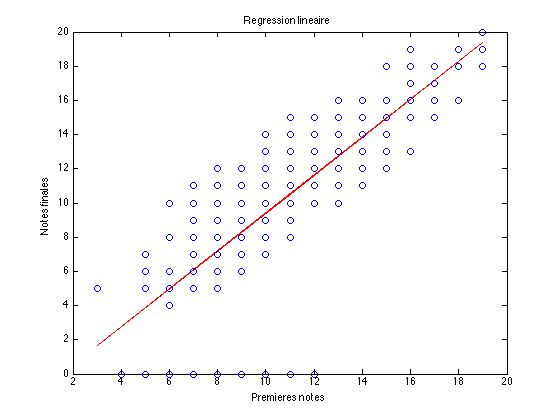
\includegraphics[scale=0.5]{Images/fig6.png}
\caption{Régression linéaire de la troisième note en fonction de la première}
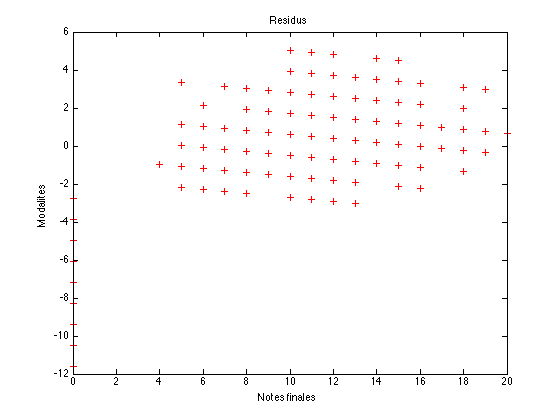
\includegraphics[scale=0.5]{Images/fig7.png}
\caption{Résidus selon les notes finales observées}
\end{figure}

\begin{figure}[h]
\centering
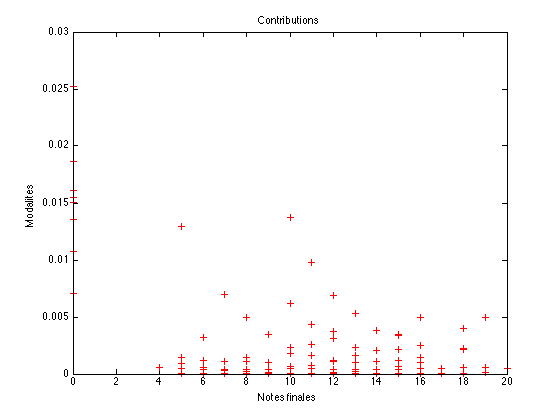
\includegraphics[scale=0.5]{Images/fig8.png}
\caption{Contributions selon les notes finales}
\end{figure}

Cependant, en regardant le graphique de la régression, celui des résidus, et celui des contributions, on remarque la présence de points aberrants correspondants tous aux notes égales à zéro. Ces points ne sont pas aberrants en soi étant donné que le zéro fait partie de l'échelle de notation. Cependant ces points ont tendance à faire chuter la qualité de la régression. C'est pourquoi après avoir réalisé une nouvelle régression avec l'absence de ces notes nous obtenons de nouveaux paramètres et un coefficient de détermination bien meilleur : $a=0,8883$ ;  $b=1,5134$ et $R^2=0,7953$.

\begin{figure}[h]
\centering
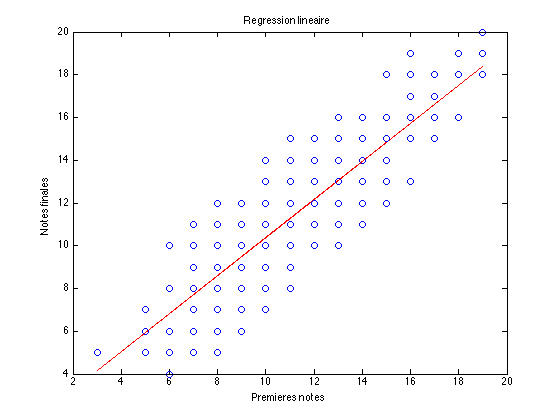
\includegraphics[scale=0.55]{Images/fig9.png}
\caption{Nouvelle régression linéaire de la troisième note en fonction de la première note, sans les points aberrants}
\end{figure}

\begin{figure}[h]
\centering
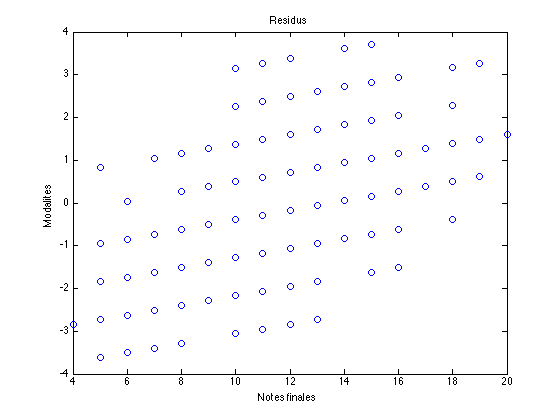
\includegraphics[scale=0.5]{Images/fig10.png}
\caption{Résidus selon les notes finales observées, sans les points aberrants}
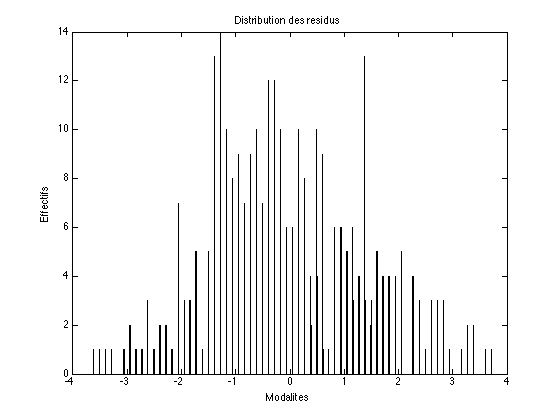
\includegraphics[scale=0.5]{Images/fig11.png}
\caption{Distribution des résidus, sans les points aberrants}
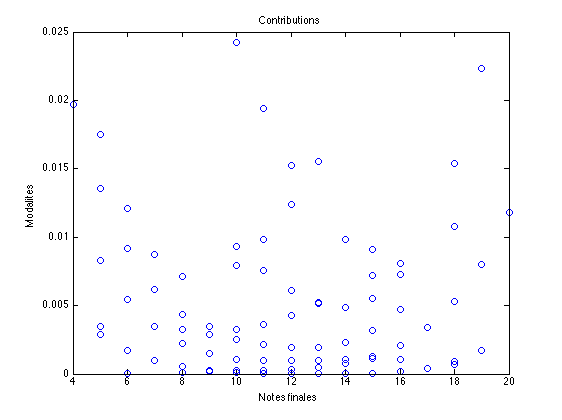
\includegraphics[scale=0.45]{Images/fig12.png}
\caption{Contributions selon les notes finales, sans les points aberrants}
\end{figure}
\FloatBarrier
Avec l'appui de ces quelques graphiques et du coefficient de détermination nous nous apercevons que le modèle linéaire est le bon. En effet, $R^2$ est plutôt proche de 1, les résidus et les contributions sont homogènes, il n'y a donc plus de points aberrants et la distribution des résidus est normale (loi gaussienne). Tous ces facteurs tendent à montrer que la prédiction de la note finale, à l'aide de la première note des élèves, est tout à fait possible. Voyons à présent s'il en est de même avec la deuxième note.
\FloatBarrier

\subsubsection{Seconde régression}
\paragraph{Régression simple :  } Peut-on prédire les notes finales des élèves à l'aide de leur deuxième note ?~\\
\begin{itemize}
\item Variable explicative : \texttt{Mat\_G2} c'est-à-dire celle contenant les deuxièmes notes des élèves.
\item Variable à expliquer : \texttt{Mat\_G3} c'est-à-dire celle contenant les notes finales des élèves.
\end{itemize}


\begin{figure}[h]
\centering
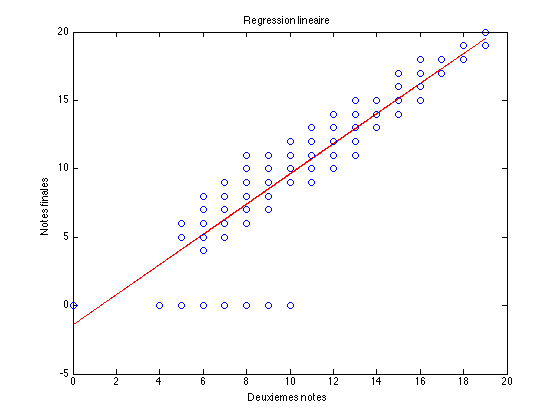
\includegraphics[scale=0.5]{Images/fig13.png}
\caption{Régression linéaire de la troisième note en fonction de la seconde}
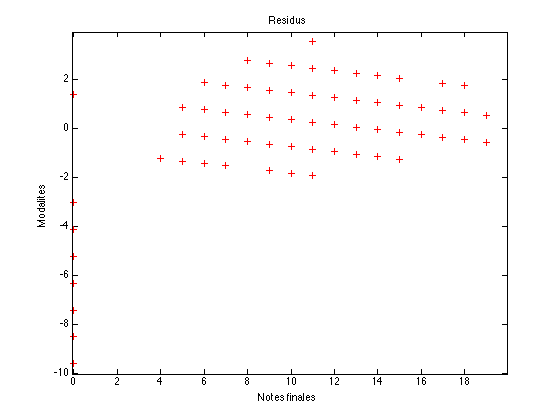
\includegraphics[scale=0.5]{Images/fig14.png}
\caption{Résidus selon les notes finales observées}
\end{figure}

\begin{figure}[h]
\centering
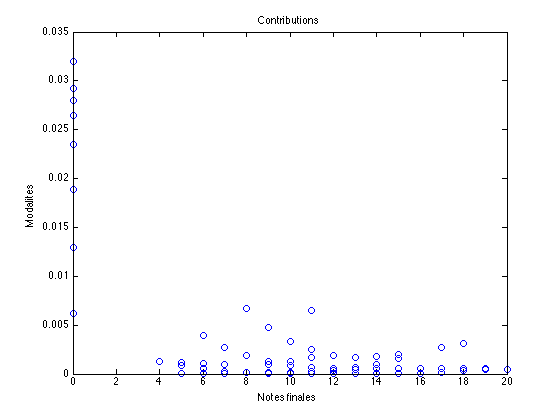
\includegraphics[scale=0.55]{Images/fig15.png}
\caption{Contributions selon les notes finales}
\end{figure}

\FloatBarrier
Une fois la régression réalisée nous nous apercevons une nouvelle fois que les notes égales à 0 viennent fausser notre régression. Cependant les paramètres et le coefficient de détermination restent tout à fait corrects : $a=1,1021$ ; $b=-1,3928$ et  $R^2=0,8188$. En effet on s'aperçoit que cette régression est de meilleure facture que la précédente, même en y laissant les notes égales à 0. Voyons à présent la qualité de cette régression en y enlevant ces notes.

\begin{figure}[h]
\centering
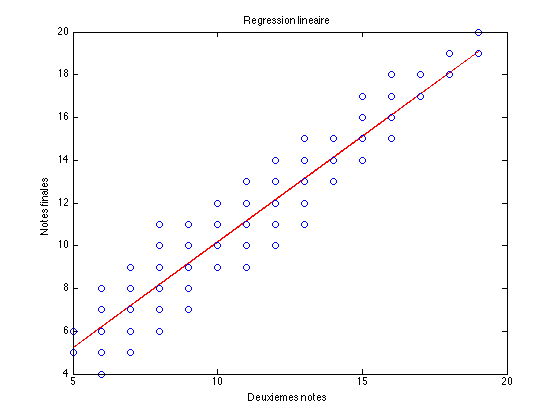
\includegraphics[scale=0.5]{Images/fig16.png}
\caption{Nouvelle régression linéaire de la troisième note en fonction de la seconde note, sans les points aberrants}
\end{figure}

\begin{figure}[h]
\centering
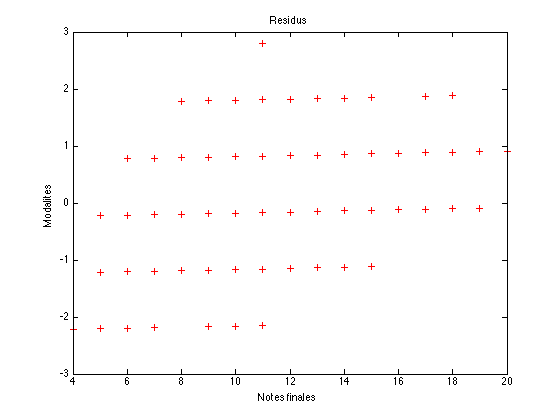
\includegraphics[scale=0.6]{Images/fig17.png}
\caption{Résidus selon les notes finales, sans les points aberrants}
\end{figure}

\begin{figure}[h]
\centering
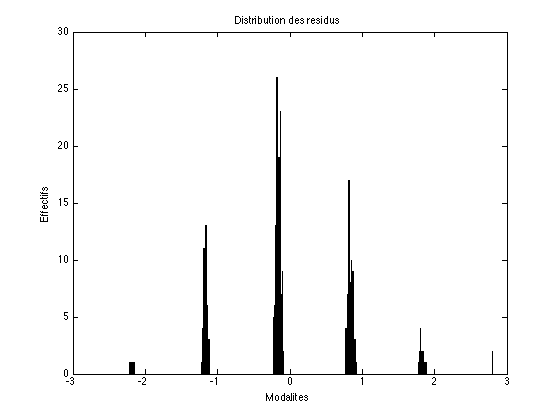
\includegraphics[scale=0.6]{Images/fig18.png}
\caption{Distribution des résidus selon les notes finales observées, sans les points aberrants}
\end{figure}

\begin{figure}[h]
\centering
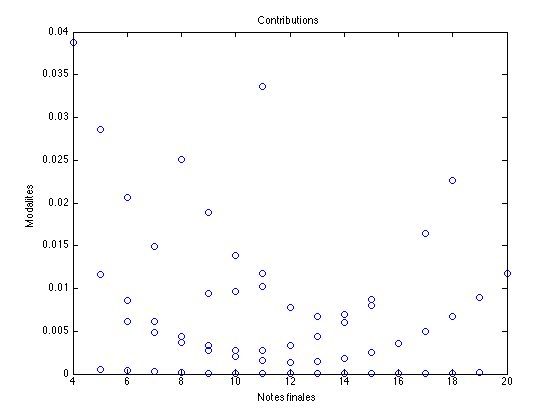
\includegraphics[scale=0.7]{Images/fig19.png}
\caption{Contributions selon les notes finales, sans les points aberrants}
\end{figure}\FloatBarrier



On obtient donc de nouveaux paramètres et, comme on pouvait s'y attendre, un coefficient de détermination meilleur : $a=0,9903$ ; $b=0,2753$ et  $R^2=0,9323$. De plus, l'étude de ces graphiques nous montre, comme lors de la régression précédente, que le modèle linéaire est excellent et que nous sommes capables de prédire la note finale, à l'aide de la deuxième note des élèves. Cependant, on peut ajouter que cette régression est bien meilleure que la précédente. En effet, le coefficient de détermination est passé de $0,7953$ à $0,9323$ ce qui signifie que la deuxième note des élèves est plus représentative de la note finale que la première. Il vaut donc mieux utiliser cette seconde note pour prédire la note finale. Mais serait t-il possible d'avoir une meilleure prédiction en utilisant à la fois la première et la deuxième note des élèves ?
 
\subsubsection{Troisième régression} 

\paragraph{Régression multiple : } Peut-on prédire les notes finales des élèves à l'aide de leurs premières et deuxième notes ?~\\

\begin{itemize}
\item Variables explicatives : \texttt{Mat\_G1} c'est-à-dire celle contenant la première note de chaque élève et \texttt{Mat\_G2} c'est-à-dire celle contenant la deuxième note de chaque élève.
\item Variable à expliquer : \texttt{Mat\_G3} c'est-à-dire celle contenant la note finale des élèves.
\end{itemize}

Une fois cette régression réalisée on obtient les paramètres et le coefficient de détermination suivants : $a_1=0,1533$ ; $a2=0,9869$ ; $b=-1,83$ et $R^2=0,8222$.

\begin{figure}[h]
\centering
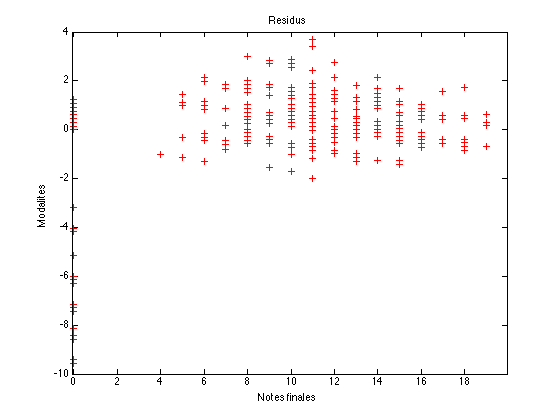
\includegraphics[scale=0.4]{Images/fig20.png}
\caption{Résidus selon les notes finales}
\end{figure}

\begin{figure}[h]
\centering
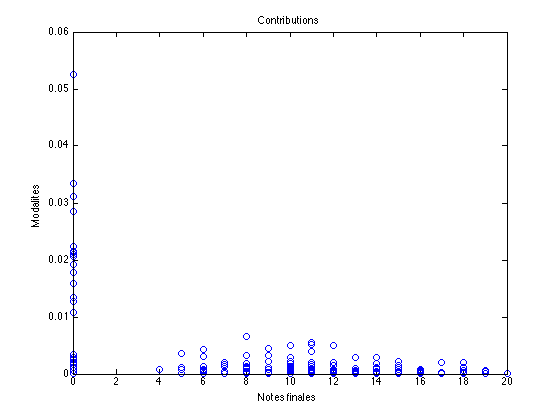
\includegraphics[scale=0.4]{Images/fig21.png}
\caption{Contribution selon les notes finales}
\end{figure}\FloatBarrier

On remarque une nouvelle fois la présence de ces notes égales à 0 qui viennent diminuer la qualité de la régression. Malgré cela la régression reste assez correcte avec un coefficient de détermination plutôt proche de 1. Cette régression est même de meilleure qualité que la première mais elle ne parvient pas à concurrencer la deuxième (lorsque l'on a retiré les points aberrants de la seconde régression). Voyons maintenant le résultat en enlevant ces points aberrants.

\begin{figure}[h]
\centering
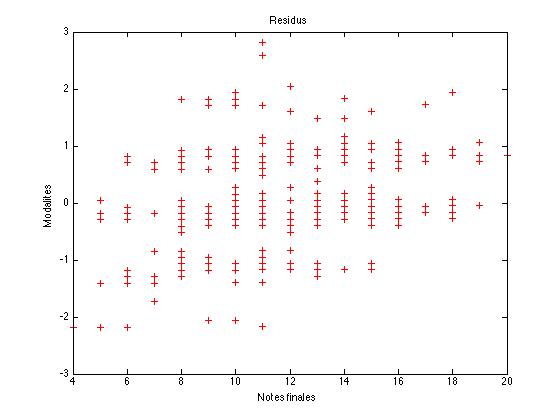
\includegraphics[scale=0.55]{Images/fig22.png}
\caption{Résidus selon les notes finales, sans les points aberrants}
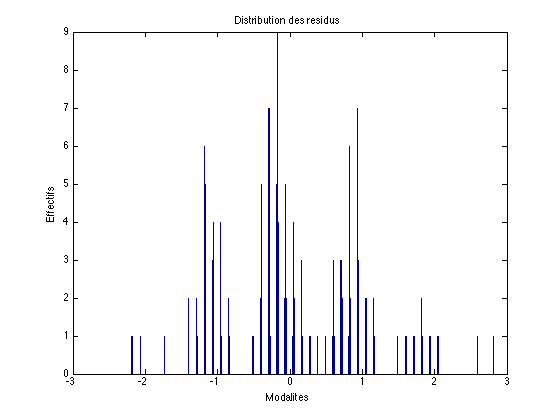
\includegraphics[scale=0.55]{Images/fig23.png}
\caption{Distribution des résidus selon les notes finales, sans les points aberrants}
\end{figure}

\begin{figure}[h]
\centering
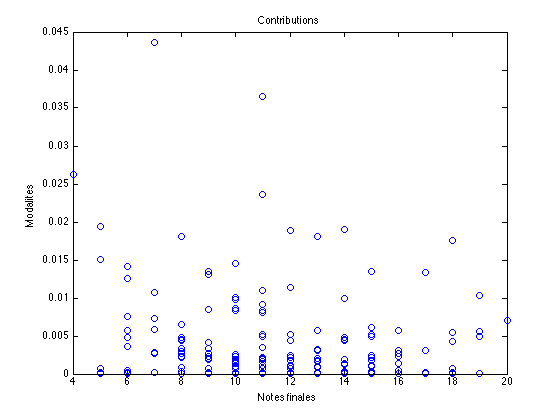
\includegraphics[scale=0.55]{Images/fig24.png}
\caption{Contributions selon les notes finales, sans les points aberrants}
\end{figure}

\FloatBarrier
On obtient les paramètres suivants : $a_1=0,1117$ ; $a_2=0,8866$ ; $b=0,1948$ ainsi qu'un coefficient de détermination très bon : $R^2=0,9347$. Une fois de plus, on s’aperçoit à l'aide de ces quelques graphiques que le modèle linéaire est très bien adapté à la situation et que l'utilisation des deux premières notes permet de prédire avec le plus de précision la note finales des élèves. La régression linéaire multiple est donc la mieux adaptée à notre problème et elle nous donne la formule suivante pour tenter de prédire la note finale des élèves si cette note n'est pas égale à 0 :
$$ y = 0,1117\cdot x_1 + 0,8866\cdot x_2 + 0,1948$$ avec $y$ la note finale, $x_1$ la première note et $x_2$ la seconde note.


\subsection{Comparaison de boites à moustache}
Lors de l'Analyse en Composantes Principales, nous avions conclu que les variables \texttt{Medu} et \texttt{Fedu} étaient corrélées positivement avec la note finale des élèves tandis que les variables \texttt{Failures} et \texttt{Age} étaient corrélées négativement avec cette dernière. Pour essayer de confirmer ces informations nous allons faire une comparaison de boites à moustache pour voir si les indicateurs (moyenne, médiane, et quartiles) diminuent ou augmentent en fonction des modalités des variables.

\paragraph{La variable \texttt{Failures}}~\\\indent
Après avoir séparé les élèves en fonction de leur nombre de redoublements nous avons obtenu les boites à moustaches suivantes.
\begin{figure}[h]
\centering
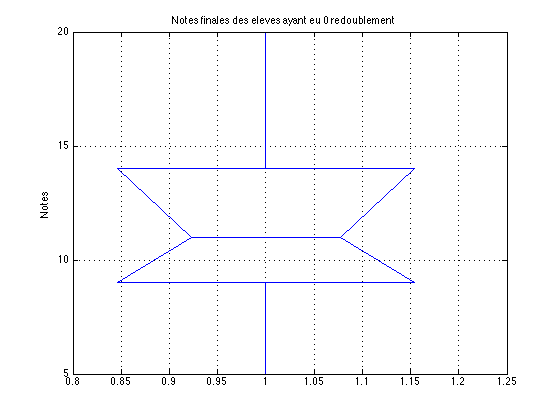
\includegraphics[scale=0.45]{Images/fig25.png}
\caption{Boîte à moustache des notes finales des élèves n'ayant jamais redoublé}
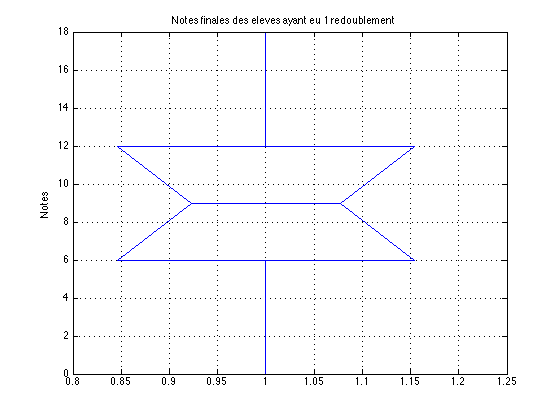
\includegraphics[scale=0.45]{Images/fig26.png}
\caption{Boîte à moustache des notes finales des élèves ayant redoublé une fois}
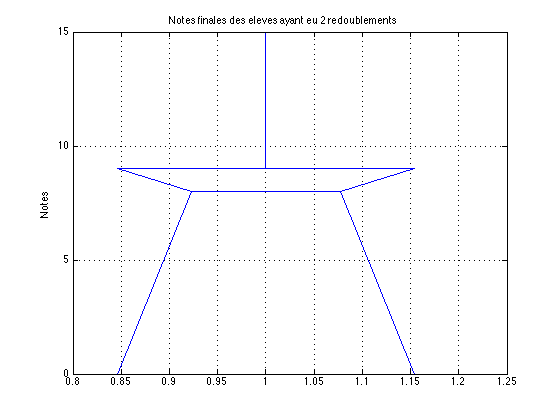
\includegraphics[scale=0.45]{Images/fig27.png}
\caption{Boîte à moustache des notes finales des élèves ayant redoublé deux fois}
\end{figure}\FloatBarrier

\begin{figure}[h]
\centering
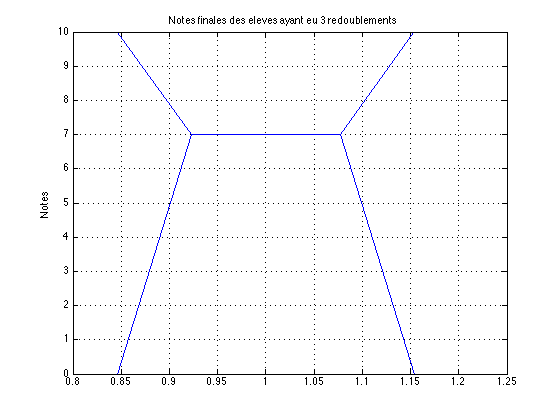
\includegraphics[scale=0.45]{Images/fig28.png}
\caption{Boîte à moustache des notes finales des élèves ayant redoublé trois fois}
\end{figure}



On constate que les principaux indicateurs (médiane et quartiles) ont tendance à diminuer plus le nombre de redoublement des élèves augmente. Ceci vient donc confirmer la thèse de la corrélation négative entre le nombre de redoublements des élèves et leurs notes finales. L'histogramme suivant concernant les moyennes des notes obtenues par chacun des groupes vient appuyer ce phénomène.

\begin{figure}[h]
\centering
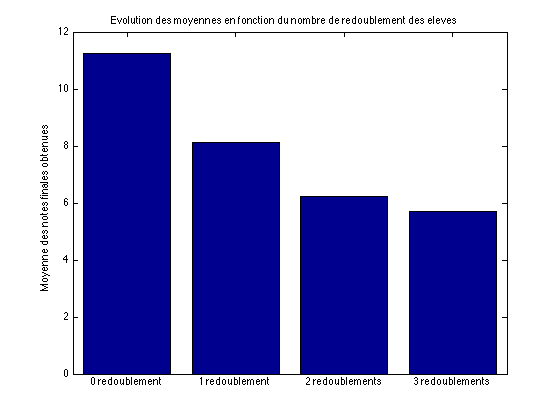
\includegraphics[scale=0.6]{Images/fig29.png}
\caption{Evolution des moyennes des élèves en fonction de leur nombre de redoublement}
\end{figure}
Nous pouvons donc affirmer que le nombre de redoublements a bien un effet négatif sur la note finale obtenue par les élèves. Plus le nombre de redoublements des élèves est élevé et plus leur note finale sera faible et inversement.

\paragraph{Les variables \texttt{Medu} et \texttt{Fedu}}~\\\indent
Après avoir séparé les élèves en fonction du niveau d'éducation de leurs parents, on constate en comparant les boites à moustaches suivantes, que les médianes et quartiles des différents échantillons tendent à augmenter à mesure que le niveau d'éducation des parents des élèves augmente. De même, l'évolution des moyennes reflète parfaitement ce phénomène et montre qu'il existe un lien évident entre les notes finales des élèves et le niveau d'éducation de leurs parents. Malheureusement, nous n'avons pas pu représenter le niveau d'éducation 0 étant donné que les élèves concernés étaient très peu nombreux. Cela ne nous permettait donc pas de les représenter au travers de leurs notes dans une boite à moustache.
\begin{figure}[h]
\centering
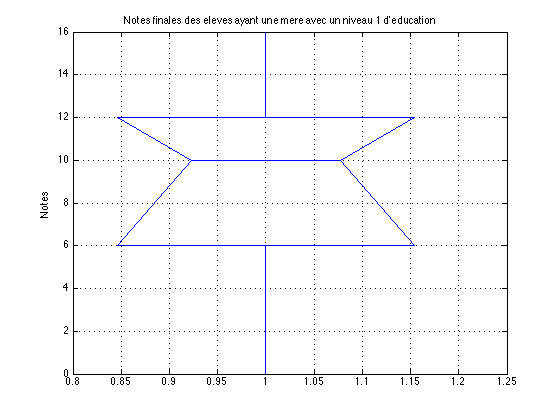
\includegraphics[scale=0.45]{Images/fig30.png}
\caption{Boîte à moustache des notes finales des élèves ayant une mère avec un niveau 1 d'éducation}
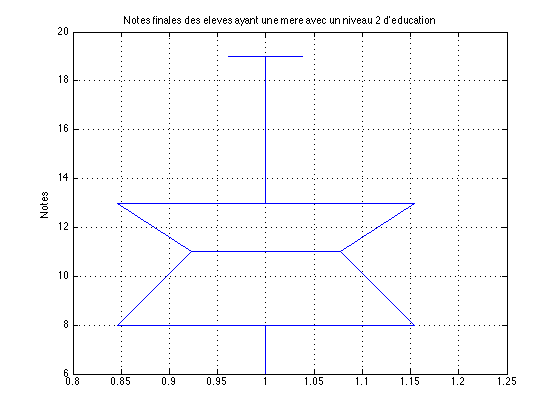
\includegraphics[scale=0.45]{Images/fig31.png}
\caption{Boîte à moustache des notes finales des élèves ayant une mère avec un niveau 2 d'éducation}
\end{figure}
\begin{figure}[h]
\centering
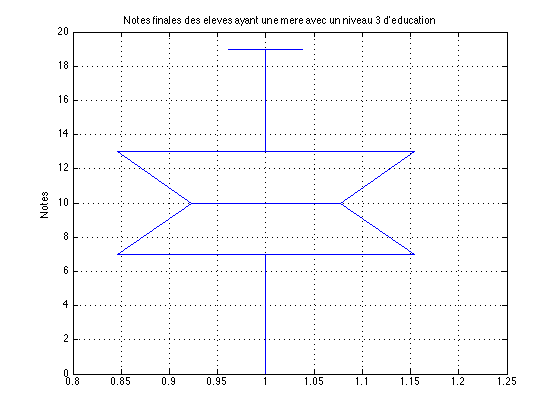
\includegraphics[scale=0.45]{Images/fig32.png}
\caption{Boîte à moustache des notes finales des élèves ayant une mère avec un niveau 3 d'éducation}
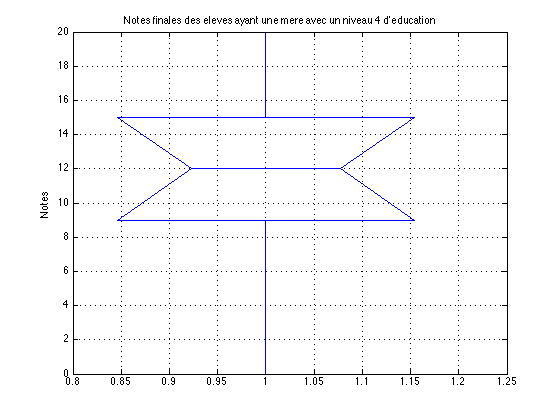
\includegraphics[scale=0.45]{Images/fig33.png}
\caption{Boîte à moustache des notes finales des élèves ayant une mère avec un niveau 4 d'éducation}
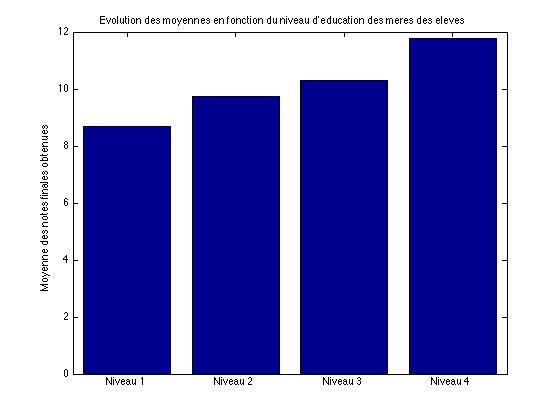
\includegraphics[scale=0.45]{Images/fig34.png}
\caption{Evolution des moyennes des élèves en fonction du niveau d'éducation des mères des élèves}
\end{figure}
\begin{figure}[h]
\centering
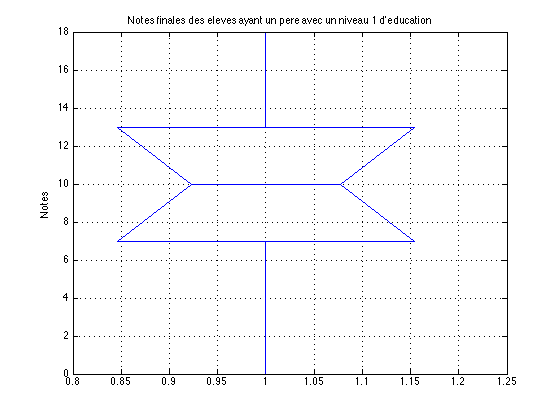
\includegraphics[scale=0.45]{Images/fig35.png}
\caption{Boîte à moustache des notes finales des élèves ayant un père avec un niveau 1 d'éducation}
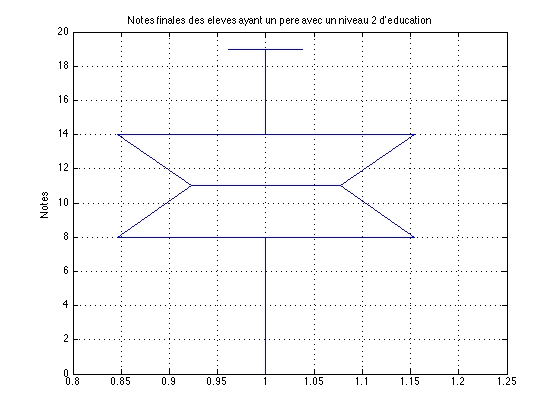
\includegraphics[scale=0.45]{Images/fig36.png}
\caption{Boîte à moustache des notes finales des élèves ayant un père avec un niveau 2 d'éducation}
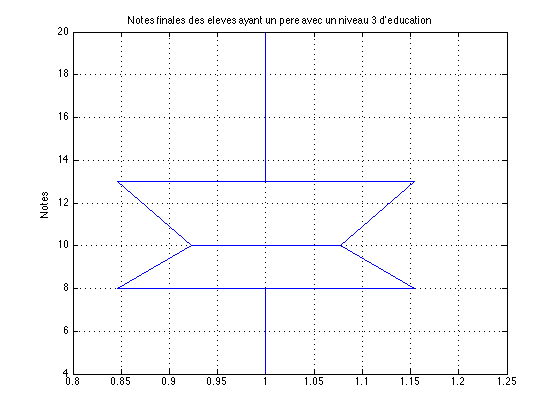
\includegraphics[scale=0.45]{Images/fig37.png}
\caption{Boîte à moustache des notes finales des élèves ayant un père avec un niveau 3 d'éducation}
\end{figure}
\begin{figure}[h]
\centering
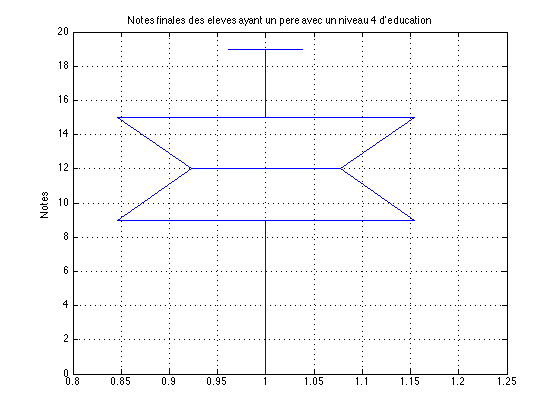
\includegraphics[scale=0.6]{Images/fig38.png}
\caption{Boîte à moustache des notes finales des élèves ayant un père avec un niveau 4 d'éducation}
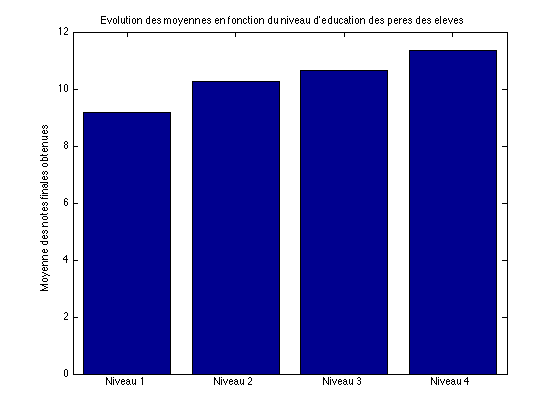
\includegraphics[scale=0.6]{Images/fig39.png}
\caption{Evolution des moyennes des élèves en fonction du niveau d'éducation des pères des élèves}
\end{figure}\FloatBarrier

Les variables \texttt{Medu} et \texttt{Fedu} sont donc bien corrélées positivement avec la variable contenant les notes finales des élèves. On est donc à présent en mesure d'affirmer que plus le niveau d'éducation des parents est élevé et plus la note finale de leur enfant sera elle aussi élevée, et inversement.

\paragraph{La variable \texttt{Age}}~\\\indent 
Nous avons dû une nouvelle fois séparer les élèves en plusieurs groupes distincts mais cette fois-ci en fonction de leurs âges. Cependant, les notes des élèves d'un âge strictement supérieur à 19 ans n'ont pu être représentées dans une boite à moustache car leur effectif était trop faible. Mais cela ne nous a en aucun cas empêché d'obtenir des résultats pour le moins satisfaisants. En effet, on remarque sur les graphiques qui vont suivre, que tous les indicateurs (moyenne médiane et quartiles) ont tendance à diminuer au fur et à mesure que l'âge des élèves augmente.

\begin{figure}[h]
\centering
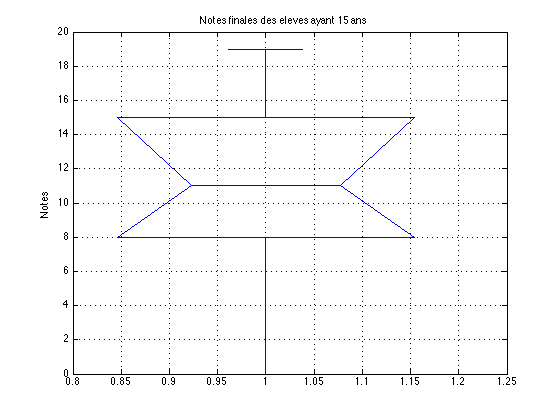
\includegraphics[scale=0.5]{Images/fig40.png}
\caption{Boîte à moustache des notes finales des élèves ayant 15 ans}
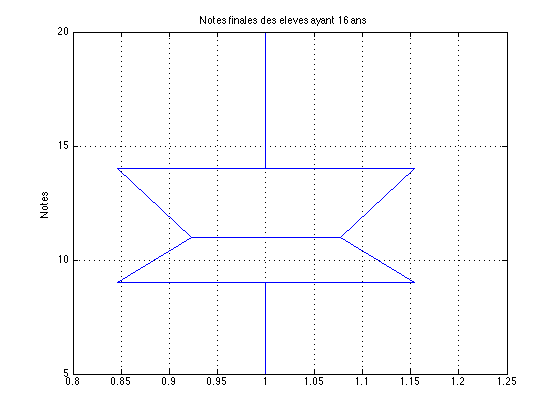
\includegraphics[scale=0.5]{Images/fig41.png}
\caption{Boîte à moustache des notes finales des élèves ayant 16 ans}
\end{figure}

\begin{figure}[h]
\centering
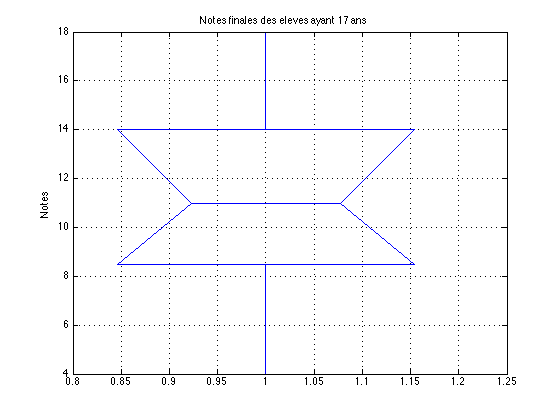
\includegraphics[scale=0.5]{Images/fig42.png}
\caption{Boîte à moustache des notes finales des élèves ayant 17 ans}
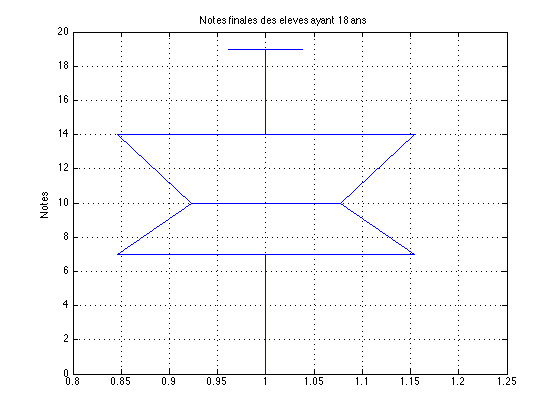
\includegraphics[scale=0.5]{Images/fig43.png}
\caption{Boîte à moustache des notes finales des élèves ayant 18 ans}
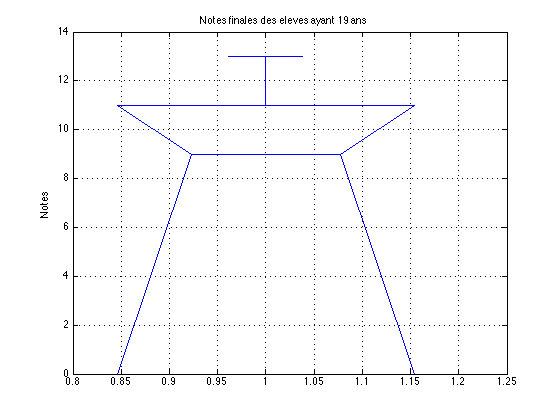
\includegraphics[scale=0.5]{Images/fig44.png}
\caption{Boîte à moustache des notes finales des élèves ayant 19 ans}
\end{figure}

\begin{figure}[h]
\centering
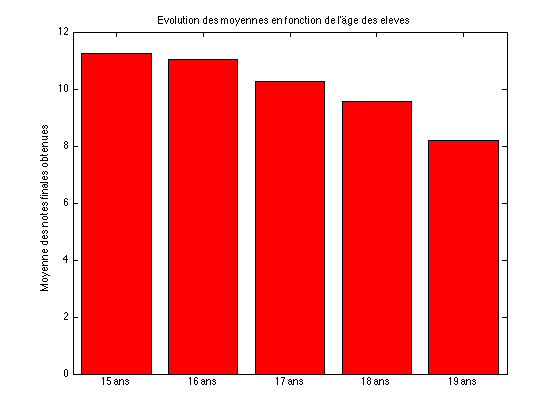
\includegraphics[scale=0.8]{Images/fig45.png}
\caption{Evolution des moyennes des élèves en fonction de leur âge}
\end{figure}\FloatBarrier

Nous sommes donc capables de dire que l'âge des élèves est corrélé négativement avec leur note finale. Ce qui signifie que plus l'âge des élèves est élevé et plus leur note finale sera faible et inversement. Ceci paraît logique car le nombre de redoublements a un rapport direct avec l'âge de l'élève. En effet, si on a déjà redoublé, on est plus vieux que ses camarades de classe, et de la même manière, si on est plus vieux, cela a de très fortes chances de signifier que l'on a déjà redoublé. De plus, comme le nombre de redoublements influence négativement la note finale alors il est très probable que l'âge en fasse de même.

Ce traitement de données nous a donc permis de tirer plusieurs enseignements. Tout abord nous avons vu que nous étions capables de prédire les notes finales des élèves (si celles-ci ne sont pas égales à 0) avec l'aide des deux premières notes obtenues par ces élèves. Par ailleurs, nous avons trouvé, avec les moyens qui sont les nôtres, que 4 variables avaient une influence sur la note finale obtenue par les élèves. En effet, nous avons découvert que \texttt{Medu} et \texttt{Fedu} étaient corrélées positivement avec la note finale, tandis que \texttt{Failures} et \texttt{Age} influençaient négativement cette dernière. Ces variables sont au nombre de 4 car nous avons fait le choix de ne tester que les variables ayant le plus de chances d'être corrélées (positivement ou négativement) avec la variable contenant les notes finales obtenues par les élèves. Ce qui signifie que des variables non traitées peuvent avoir elles aussi une influence sur la note finales des élèves.

\newpage
\FloatBarrier
%%%%%%%%%%%%%%%%%%%%%%%%%%%%%%%%%%Partie 2
\section{Tests}
%%%%%%%%%%%   Chi2
\subsection{Tests du $\chi ^2$}
Nous réaliserons ici différents tests. Cependant, le raisonnement étant toujours analogue, nous n'allons détailler qu'une première fois les calculs.
\subsubsection{Test du $\chi^2$ détaillé sur les variables \texttt{Internet} et \texttt{Studytime}}
Pour réaliser des tests du $\chi^2$, il faut choisir deux variables qualitatives. Dans notre jeu de données, la plupart des variables sont qualitatives et il nous serait long et fastidieux de tester toutes les variables deux par deux. Ainsi, avec les avals de Messieurs \textsc{Delporte}, \textsc{Canu} et \textsc{Rousselle}, nous avons décidé de ne tester que des couples de variables qui pouvait \emph{a priori} être liées. Ainsi, comme premier test, nous avons décidé de tester les variables \texttt{Internet}, qui indique si un étudiant a accès à un Internet ou non, et \texttt{Studytime}, qui est une variable de catégories selon le temps que passe l'élève à étudier par semaine. Nous allons, une fois encore, développer les calculs réalisés à partir des données du fichier \texttt{student-mat.csv} mais le raisonnement est totalement analogue avec les données issues de l'autre fichier.

\paragraph{Etape 1 : construire le tableau de contingence}~\\\indent
Tout d'abord, on fixe nos hypothèses de départ : 
\begin{itemize}
\item[\textbullet] \og $H_0$ : le fait qu'un élève ait accès à Internet n'est pas en lien avec le temps qu'il passe à étudier chaque semaine\fg.
\item[\textbullet] \og $H_1$ : le fait qu'un élève ait accès à Internet est lié avec le temps qu'il passe à étudier chaque semaine\fg.
\end{itemize}

Ensuite, on construit le tableau de contingence $O$ des observations. On réalise pour cela plusieurs boucles, en passant par une matrice temporaire qui regroupe les deux variables à étudier, pour chercher les effectifs d'individus qui correspondent respectivement aux différents couples de variables.

\begin{lstlisting}[firstnumber=15,caption={Extrait des boucles permettant de construire le tableau de contingence du test du $\chi^2$}]
    temp=[TabModMat_Internet , Mat_Studytime];
    
    O = zeros(2,4); % 2 lignes pour 'internet' et 4 colonnes pour 'studytime'
    
    ind=[]; %Pour [0,1]
    for i=1:length(temp)
        if temp(i,:)==[0,1]
            ind=[ind i];
        end
    end
   O(1,1)=length(ind);
   
    ind=[]; %Pour [0,2]
    for i=1:length(temp)
        if temp(i,:)==[0,2]
            ind=[ind i];
        end
    end
   O(1,2)=length(ind);
   
    ind=[]; %Pour [0,3]
    for i=1:length(temp)
        if temp(i,:)==[0,3]
            ind=[ind i];
        end
    end
   O(1,3)=length(ind);
   
   % Et ainsi de suite pour les autres couples
\end{lstlisting}

A la fin, on obtient le tableau de contingence (contenant des effectifs) suivant :

\begin{table}[h] \centering \caption{Tableau de contingence du test de $\chi^2$ entre les variables \texttt{Internet} et \texttt{Studytime}}
\begin{tabular}{|c|c|c|c|c|}
  \hline
 	\backslashbox{\textbf{\emph{Internet}}}{\textbf{\emph{Studytime}}}& \textbf{Moins de 2 heures} & \textbf{Entre 2 et 5 heures} & \textbf{Entre 5 et 10 heures} & \textbf{Plus de 10 heures}\\
  \hline
          
          \textbf{Non} & 19 & 37 & 6 & 4\\\hline
          \textbf{Oui} & 86 & 161 & 59 & 23 \\\hline
          \end{tabular}
\end{table}

\paragraph{Etape 2 : on calcule les marginales}~\\\indent
On calcule les marginales du tableau de contingence.
\begin{lstlisting}[firstnumber = 86, caption={Calcul des marginales du tableau de contingence pour le test du $\chi^2$}]
    [I,J]=size(O); %[2,4]
    nI=sum(O'); %profil ligne = [66 329]
    nJ=sum(O); %profil colonne = [105 198 65 27]
    n=sum(sum(O)); % = 395
 \end{lstlisting}
 
 \paragraph{Etape 3 : on calcule les $T_{i,j}$ pour créer le tableau des effectifs théoriques (en supposant l'indépendance)}~\\\indent
 On calcule les $T_{i,j}=n\cdot p_i\cdot p_j$ avec le code suivant :
 \begin{lstlisting}[firstnumber=92,caption={Calcul des effectifs théoriques pour le test du $\chi^2$}]
    T=(nI'*nJ)/n; % Effectifs theoriques <==> Tij=P(i.)*P(.j)*n
                                         %= Ni./n * N.j/n * n
    % T/n donne les pourcentages
\end{lstlisting}

\paragraph{Etape 4 : on calcule la distance du $\chi^2$}~\\\indent
La distance du $\chi^2$ entre les effectifs observés dans le tableau de contingence et les effectifs théoriques est défini par la formule :
$$D(O,T)=\sum_{i=1}^{I}\sum_{j=1}^{J}\frac{\left(O_{i,j}-T_{i,j}\right)^2}{T_{i,j}} $$
On la calcule en \emph{Matlab} par le code suivant :
 \begin{lstlisting}[firstnumber=97,caption={Calcul de la distance du $\chi^2$}]
    D= sum(sum((O-T).^2./T)); %Distance du Chi2 : 3.3831
\end{lstlisting}

\paragraph{Etape 5 : calcul du degré de liberté du $\chi^2$}~\\\indent
Le degré de liberté du $\chi^2$ est donné par la relation : $ddl = (I-1)\cdot(J-1)$. Ainsi, dans notre cas : \lstinline{ddl=(I-1)*(J-1); %3}.

\paragraph{Etape 6 : On regarde dans les tables de la loi $\chi^2$ à $ddl$ degrés de liberté}~\\\indent
Soit $Z$ une variable aléatoire suivant la loi $\chi^2$ à $ddl$ degrés de liberté. On cherche la P-Valeur, définie ici par :
$$ pval=P(Z\geq D(O,T))$$
Ainsi, pour notre cas, on obtient la P-Valeur par le code suivant :
\begin{lstlisting}[firstnumber=103,caption={Calcul de la P-Valeur avec les tables de la loi de $\chi2$}]
pval=1-chi2cdf(3.3831,3) % pval =  0.33624
\end{lstlisting}


\paragraph{Etape 7 : conclure}~\\\indent
On remarque que $pval = 0,33624 \geq 0,05$, on rejette donc $H_0$ et il y a lieu de remettre en cause l'indépendance des variables \texttt{Internet} et \texttt{Studytime}.

~\\
Après avoir réalisé le même test sur le second fichier avec ces deux variables, nous aboutissons à la même conclusion.


\subsubsection{Test du $\chi^2$ sur les variables \texttt{Romantic} et \texttt{Walc}}
On réalise à présent un test du $\chi^2$ sur les variables \texttt{Romantic}, qui indique si l'élève était dans une relation amoureuse au moment de l'enquête, et \texttt{Walc} qui indique la consommation hebdomadaire d'alcool de l'élève. On n'indiquera pas les calculs, ceux-ci étant similaires à ceux réalisés précédemment. En revanche, tous les calculs sont disponibles dans le fichier joint dans l'archive, intitulé \texttt{Test\_Chi2.m}. Par ailleurs, les résultats qui vont être énoncés ici seront ceux issus des données du fichier \texttt{student-mat.csv}. 

Le tableau de contingence obtenu est le suivant. Pour la variable \texttt{Walc} on rappelle que les modalités vont de \og 1\fg\ pour une consommation très faible à \og 5\fg\ pour une consommation importante d'alcool.
\begin{table}[h] \centering \caption{Tableau de contingence du test de $\chi^2$ entre les variables \texttt{Romantic} et \texttt{Walc}}
\begin{tabular}{|c|c|c|c|c|c|}
  \hline
 	\backslashbox{\textbf{\emph{Romantic}}}{\textbf{\emph{Walc}}}& \textbf{1} & \textbf{2} & \textbf{3} & \textbf{4} & \textbf{5}\\
  \hline
          
          \textbf{Non} & 100 & 56 & 52 &  38 & 17\\\hline
          \textbf{Oui} & 51 & 29 & 28 & 13 & 11 \\\hline
          \end{tabular}
\end{table}

On obtient alors la distance du $\chi^2$ : $D(O,T)=1.9912$, et on obtient que la P-Valeur vaut : $pval = 0.73738$. On déduit alors que, comme $pval\geq 0.05$, on rejette $H_0$ et on en déduit que les deux variables ne sont pas statistiquement indépendantes. Même constat après avoir testé ces mêmes variables dans le fichier \texttt{student-por.csv}.

\subsubsection{Test du $\chi^2$ sur les variables \texttt{Medu} et \texttt{Fedu}}
On réalise maintenant un test du $\chi^2$ sur les variables \texttt{Medu}, qui représente le niveau d'éducation de la mère, et \texttt{Fedu} qui représente le niveau d'éducation du père. On n'indiquera pas les calculs, ceux-ci étant similaires à ceux réalisés précédemment. En revanche, tous les calculs sont disponibles dans le fichier joint dans l'archive, intitulé \texttt{Test\_Chi2.m}. Par ailleurs, les résultats qui vont être énoncés ici seront ceux issus des données du fichier \texttt{student-mat.csv}. 

Le tableau de contingence obtenu est le suivant. Se référer à la page \pageref{rap1} pour la signification des différentes modalités.
\begin{table}[h] \centering \caption{Tableau de contingence du test de $\chi^2$ entre les variables \texttt{Medu} et \texttt{Fedu}}
\begin{tabular}{|c|c|c|c|c|c|}
  \hline
 	\backslashbox{\textbf{\emph{Medu}}}{\textbf{\emph{Fedu}}}& \textbf{0} &\textbf{1} & \textbf{2} & \textbf{3} & \textbf{4} \\
  \hline
          
            \textbf{0}&   0 &    1 &    2 &    0 &    0 \\\hline
     	\textbf{1} &1   & 37    &15   &  5     &1\\\hline
    \textbf{2} & 0   & 28    &51    &17     &7\\\hline
     \textbf{3} & 0  &  15   & 28  &  38  &  18\\\hline
     \textbf{4} &1    & 1   & 19  &  40    &70  \\\hline        \end{tabular}
\end{table}

On obtient alors la distance du $\chi^2$ : $D(O,T)=199.9773$, et on obtient que la P-Valeur vaut : $pval = 0$. On déduit alors que, comme $pval\leq 0.05$, On garde donc $H_0$ : il n'y a pas lieu de remettre en cause l'indépendance des variables \texttt{Medu} et \texttt{Fedu}. Même constat après avoir testé ces mêmes variables dans le fichier \texttt{student-por.csv}.

\subsubsection{Test du $\chi^2$ sur les variables \texttt{Mjob} et \texttt{Fjob}}
On réalise ici un test du $\chi^2$ sur les variables \texttt{Mjob}, qui représente le type d'emploi de la mère, et \texttt{Fjob} qui représente le type d'emploi du père. On n'indiquera pas les calculs, ceux-ci étant similaires à ceux réalisés précédemment. En revanche, tous les calculs sont disponibles dans le fichier joint dans l'archive, intitulé \texttt{Test\_Chi2.m}. Par ailleurs, les résultats qui vont être énoncés ici seront ceux issus des données du fichier \texttt{student-mat.csv}. 

Le tableau de contingence obtenu est le suivant. Se référer à la page \pageref{rap2} pour la signification des différentes modalités.
\begin{table}[h] \centering \caption{Tableau de contingence du test de $\chi^2$ entre les variables \texttt{Mjob} et \texttt{Fjob}}
\begin{tabular}{|c|c|c|c|c|c|}
  \hline
 	\backslashbox{\textbf{\emph{Mjob}}}{\textbf{\emph{Fjob}}}& \textbf{0} &\textbf{1} & \textbf{2} & \textbf{3} & \textbf{4} \\
  \hline
          
            \textbf{0}&       7 &    2  &  33   & 15  &   2\\\hline
    \textbf{1}& 0     &6   & 17    &10     &1 \\\hline
    \textbf{2} &5 &    2  & 104  &  24 &    6\\\hline
     \textbf{3}& 6  &    4   & 42  &  43  &   8\\\hline
     \textbf{4}& 2 &    4    &21 &   19   & 12\\\hline
 \end{tabular}
\end{table}

On obtient alors la distance du $\chi^2$ : $D(O,T)=73.3809$, et on obtient que la P-Valeur vaut : $pval = 2.5336\cdot 10^{-9}$. On déduit alors que, comme $pval\leq 0.05$, On garde donc $H_0$ : il n'y a pas lieu de remettre en cause l'indépendance des variables \texttt{Mjob} et \texttt{Fjob}. Même constat après avoir testé ces mêmes variables dans le fichier \texttt{student-por.csv}.

%
\subsubsection{Test du $\chi^2$ sur les variables \texttt{Dalc} et \texttt{Walc}}
On réalise ici un test du $\chi^2$ sur les variables \texttt{Dalc}, qui représente la consommation quotidienne d'alcool de l'élève, et \texttt{Walc} qui représente sa consommation d'alcool hebdomadaire. On n'indiquera pas les calculs, ceux-ci étant similaires à ceux réalisés précédemment. En revanche, tous les calculs sont disponibles dans le fichier joint dans l'archive, intitulé \texttt{Test\_Chi2.m}. Par ailleurs, les résultats qui vont être énoncés ici seront ceux issus des données du fichier \texttt{student-mat.csv}. 

Le tableau de contingence obtenu est le suivant. Se référer à la page \pageref{rap3} pour la signification des différentes modalités.
\begin{table}[h] \centering \caption{Tableau de contingence du test de $\chi^2$ entre les variables \texttt{Dalc} et \texttt{Walc}}
\begin{tabular}{|c|c|c|c|c|c|}
  \hline
 	\backslashbox{\textbf{\emph{Dalc}}}{\textbf{\emph{Walc}}}& \textbf{1} &\textbf{2} & \textbf{3} & \textbf{4} & \textbf{5} \\
  \hline
          
            \textbf{1}  & 150   & 65  &  42  &  15 &    4\\\hline
           \textbf{2}& 1  &  18&    29   & 22 &    5\\\hline
    	      \textbf{3}&  0 &    1 &    8  &  11  &   6\\\hline
           \textbf{4} & 0  &   1  &   1  &   3   &  4\\\hline
          \textbf{5} & 0   &  0  &   0 &    0   &  9\\\hline
 \end{tabular}
\end{table}

On obtient alors la distance du $\chi^2$ : $D(O,T)=287.0019$, et on obtient que la P-Valeur vaut : $pval = 0$. On déduit alors que, comme $pval\leq 0.05$, On garde donc $H_0$ : il n'y a pas lieu de remettre en cause l'indépendance des variables \texttt{Dalc} et \texttt{Walc}. Même constat après avoir testé ces mêmes variables dans le fichier \texttt{student-por.csv}.

Ici, le résultat paraît assez surprenant, car les variables semblent \emph{a priori} pouvoir être liées. Pourtant, il semble bien au vu des résultats que la consommation quotidienne d'alcool et la consommation hebdomadaire ne soient pas liées.

%%%%%%%%%%%%%%    Student

\subsection{Tests de \textsc{Student}}
Pour réaliser des tests de \textsc{Student}, il faut choisir deux variables quantitatives. Dans notre jeu de données, seules deux variables représentent réellement des quantités : \texttt{Age} et \texttt{Absences}. En effet, si nous transformons toutes les autres données (notamment celles qui sont d'origine en chaîne de caractères) en valeurs numériques, elles ne représentent pour autant pas des quantités, et un test de \textsc{Student} n'a sur ces variables aucun intérêt. Par ailleurs, la plupart de nos variables représentent des catégories. En effet, à l'image de \texttt{Traveltime}, les valeurs que va prendre la variable seront \og 1 \fg\ si le temps de voyage de l'élève est compris dans un intervalle de temps inférieur à 15 minutes, \og 2 \fg si le temps est compris entre 15 et 30 minutes... La variable n'est pas quantitative dans le sens où elle ne représente pas réellement le temps de voyage : la variable n'est pas égale à 22 si l'élève met 22 minutes pour venir à l'école. Ainsi, il paraît assez peu intéressant de réaliser un test de \textsc{Student} sur de telles variables.

~\\ Seules deux variables correspondent à des variables réellement quantitatives, l'âge de l'étudiant et son taux d'absentéisme, comme nous l'avons dit un peu plus tôt. Nous allons alors soumettre ces deux variables au test de \textsc{Student}. Une fois de plus, nous ne représentons que le test de \textsc{Student} réalisé sur les données du fichier \texttt{student-mat.csv}, mais les calculs sont identiques dans le fichier lié aux notes obtenues en cours de langue portugaise.

\paragraph{Etape 1 : formuler les hypothèses}~\\\indent
Formulons les hypothèses dont nous allons essayer de trouver celle qui représente le plus la réalité :
\begin{itemize}
\item[\textbullet] \og $H_0$ : l'âge de l'élève n'est pas en lien avec son taux d'absentéisme\fg. 
\item[\textbullet] \og $H_1$ : l'âge de l'élève est lié à son taux d'absentéisme \fg.
\end{itemize}

\paragraph{Etape 2 : poser un modèle}~\\\indent
Soit $\overline{x_{age}}$ (noté \texttt{Xb\_age} dans le programme) la variable aléatoire représentant la moyenne des âges. On a alors : 
$$ \overline{x_{age}} \sim \mathcal{N}\left( \mu_{age},\frac{\sigma_{age}^2}{n_{age}}\right)$$ 
On a alors \lstinline{Xb_age=mean(Mat_Age); % 16.6962 : age moyen}.

Par un raisonnement similaire, on a \lstinline{Xb_absences=mean(Mat_Absences); % 5.7089 : absenteisme moyen}.

On calcule alors le $\widehat{\sigma}^2$ : 
$$ \widehat{\sigma}^2 = \frac{1}{n_{\text{age}} + n_{\text{absences}}-2}\cdot \left( \sum_{i=1}^{n_{\text{age}}} \left(x_{\text{age},i} - \overline{x_{\text{age}}} \right)^2 +  \sum_{i=1}^{n_{\text{absences}}} \left(x_{\text{absences},i} - \overline{x_{\text{absences}}} \right)^2\right)$$

\begin{lstlisting}[firstnumber=28, mathescape,caption={Calcul du $\widehat{\sigma}^2$ pour le test de \textsc{Student}}]
%Calcul du Sigma2 :
            sigma2=(1/(length(Mat_Absences) + length(Mat_Age)-2));
            sigma2=sigma2*(sum((Mat_Absences-Xb_absences).^2)+sum((Mat_Age-Xb_age).^2)); 
            											$\hookrightarrow$%% 32.8389
\end{lstlisting} 

On reformule alors les hypothèses : 
\begin{itemize}
\item[\textbullet] $H_0$ : $\mu_{\text{age}} = \mu_{\text{absences}}$.
\item[\textbullet] $H_1$ : $\mu_{\text{age}}\neq \mu_{\text{absences}}$.
\end{itemize}

\paragraph{Etape 3 : exhiber la statistique du test.}~\\\indent
A ce moment, on peut calculer $t$ :
$$ t = \frac{\overline{x_{\text{age}}} - \overline{x_{\text{absences}}}}{\sqrt{\widehat{\sigma}^2 \left(\frac{1}{n_{\text{age}}} + \frac{1}{n_{\text{absences}}}\right)}}$$
et le nombre de degrés de liberté :
$$ ddl = n_{\text{age}}+n_{\text{absences}} -2$$ 

\begin{lstlisting}[firstnumber=39, mathescape,caption={Calcul de $t$ et du nombre de degrés de liberté pour le test de \textsc{Student}}]
t=(Xb_age-Xb_absences) / (sqrt(sigma2*(1/length(Mat_Age) + 1/length(Mat_Absences)))); 
										$\hookrightarrow$ %26.9452 
%Nombre de degres de liberte : 
ddl = length(Mat_Age)+length(Mat_Absences)-2; %788
\end{lstlisting}

\paragraph{Etape 4 : calculer la P-Valeur}~\\\indent
On calcule la p-valeur : 
$$pval = 2\cdot P(T\geq t)$$

\begin{lstlisting}[firstnumber=45,caption={Calcul de la P-Valeur pour le test de \textsc{Student}}]
P_val=2*(1-cdf('t',26.9452, 788)) ; %0
\end{lstlisting}

\paragraph{Etape 5 : conclure}~\\\indent
La P-Valeur étant inférieure à $\alpha = 0.05$, on garde donc l'hypothèse de départ $H_0$. Ainsi, on en déduit que l'âge des élèves n'est pas en lien avec leur taux d'absentéisme.

~\\ De prime abord, il paraissait presque évident que l'âge d'un élève n'influait pas sur son taux d'absentéisme. Le test de \textsc{Student} nous l'a alors confirmé. 

~\\\\
En réalisant les mêmes calculs avec le second fichier, on trouve $t=69.4753$, $ddl=1296$ et alors \lstinline{P_val= 2*(1-cdf('t',69.4753,1296)) %=0}. 
Pour ce second fichier, on en arrive à la même conclusion : l'âge n'influe pas sur l'absentéisme.


\newpage
\section*{Conclusion}\addcontentsline{toc}{section}{Conclusion}\thispagestyle{mine}
Ce projet nous a permis de mettre en œuvre quelques méthodes statistiques vues en cours tout en les adaptant à notre problème. Cela nous a donc appris à déceler quelles méthodes étaient les mieux adaptées à notre problématique de départ. En effet, le but de ce projet n'était pas selon nous de ressortir l’intégralité des méthodes vues en cours sans réfléchir. Nous avons souhaité rechercher quelles méthodes du cours convenaient le mieux à notre problème tout en ayant également accès à d'autres méthodes statistiques qui à nos yeux nous paraissaient intéressantes et utiles pour répondre à notre problématique. ~\\

Passons maintenant aux résultats plus concrets que nous a permis de révéler ce projet. Tout d'abord, nous avons appris grâce à quelques régressions linéaires qu'il était possible de prédire les notes finales des élèves à l'aide de leurs deux premières notes obtenues au cours de l'année. Dans un second temps, nous avons été en mesure, grâce à plusieurs méthodes (en l'occurrence ici, une analyse en composantes principales et des comparaisons de boîte à moustache), de montrer que certaines variables avaient une influence sur la note finale obtenue par les élèves. Nous avons notamment trouvé que les variables \texttt{Medu} et \texttt{Fedu} étaient corrélées positivement avec les notes finales des élèves tandis que les variables \texttt{Age} et \texttt{Failures} étaient corrélées négativement avec ces dernières. Dans un dernier temps nous avons décidé à l'aide de quelques tests de voir si certaines variables étaient liées entre elles. En effet, lors de la partie traitement nous annoncions qu'il paraissait logique que les variables \texttt{Age} et \texttt{Failures} soient liées. Cependant, nous avons prouvé à l'aide d'un test de \textsc{Student} que ce n'était pas du tout le cas. Ainsi, ce que nous pensons être logique ne reflète pas toujours la réalité. De même, alors que nous pensions que les variables \texttt{Dalc} et \texttt{Walc} pouvaient avoir un lien entre elles et que les variables \texttt{Medu} et \texttt{Fedu} semblaient être corrélées selon notre ACP. Il s'est avéré que ce que nous pensions était faux. 

En effet, nous avons été en mesure de montrer grâce au test du $\chi^2$ que les couples de variables \texttt{Dalc}/\texttt{Walc}, \texttt{Medu}/\texttt{Fedu} ainsi que d'autres comme \texttt{Romantic}/\texttt{Walc} et \texttt{Mjob}/\texttt{Fjob} n'étaient pas liées. ~\\


Bien entendu, notre étude n'est en aucun cas exhaustive étant donné que notre base de données contient un très grand nombre de variables, il nous était donc impossible de traiter toutes les relations possibles entre chacune des variables. Nous avons préféré éclairer les relations entre les variables qui nous semblaient logiques ainsi que celles qui nous paraissaient intéressantes. Cependant, chacun peut s'il le souhaite approfondir notre sujet pour le traiter en intégralité, notamment en y apportant d'autres méthodes statistiques et en testant les relations entre les variables que nous n'avons pas pu traiter.
\newpage
\lstlistoflistings\addcontentsline{toc}{section}{Liste des codes}\thispagestyle{mine}
\listoftables\addcontentsline{toc}{section}{Liste des tableaux}
\listoffigures\addcontentsline{toc}{section}{Liste des figures}


\newpage
\section*{Annexes}\addcontentsline{toc}{part}{Annexes}\pagenumbering{roman}
\subsection*{Annexe A \--- \texttt{DonneesProjetM8.m}} \addcontentsline{toc}{section}{Annexe A \--- \texttt{DonneesProjetM8.m}}
\lstinputlisting{DonneesProjetM8.m}
\newpage
\subsection*{Annexe B \--- \texttt{Traitement.m}}\addcontentsline{toc}{section}{Annexe B \--- \texttt{Traitement.m}}
\lstinputlisting{Traitement.m}
\newpage
\subsection*{Annexe C \--- \texttt{Test\_Chi2.m}}\addcontentsline{toc}{section}{Annexe C \--- \texttt{Test\_Chi2.m}}
\lstinputlisting{Test_Chi2.m}
\newpage
\subsection*{Annexe D \--- \texttt{Test\_Student.m}}\addcontentsline{toc}{section}{Annexe D \--- \texttt{Test\_Student.m}}

\lstinputlisting{Test_Student.m}
\end{document}

%% A faire : verifier les noms figures

%% modifier les tests

%% faire l'intro